%! Author = Axel
%! Date = 21/10/2024

% Preamble
\documentclass[11pt]{article}

% Packages
\usepackage{amsmath}
\usepackage{geometry}
\usepackage{fancyhdr}
\usepackage{titlesec}
\usepackage{hyperref}
\usepackage{graphicx}
\usepackage{float}
\usepackage{wasysym} % Add this line

% Geometry
\geometry{a4paper, margin=1in}

% Header and Footer
\pagestyle{fancy}
\fancyhf{}
\fancyhead[L]{\leftmark}
\fancyhead[R]{\thepage}

% Section formatting
\titleformat{\section}{\large\bfseries}{\thesection}{1em}{}
\titleformat{\subsection}{\normalsize\bfseries}{\thesubsection}{1em}{}

% Document
\begin{document}

\title{Sistemi Operativi Modulo 1 - Appunti}
\author{Axel}
\date{\today}
\maketitle

\tableofcontents
\newpage

    \usepackage{graphicx}\section{I Processi}
\subsection{Requisiti di OS}
Il  Compito fondamentale di un sistema operativo é la gestione dei processi, ovvero delle diverse computazione che si vuol
eseguire su un sistema computerizzato. Il sistema operativo deve:
\begin{itemize}
    \item permettere l'esecuzione alternata di più processi (multitasking)
    \item assegnare le risorse del sistema ai processi, e decidere se dare la CPU a un processo o meno
    \item permettere ai processi di scambiarsi informazioni
    \item permettere la sincronizzazione tra processi (es. semafori)
\end{itemize}
\subsubsection{Cos'è un processo}
Un processo è un programma in esecuzione, ovvero un'istanza di un programma in esecuzione su un computer, un certo programma
puó essere eseguito più volte, e ogni esecuzione è un processo diverso.
L'entitá che puó essere assegnata a un processore è il processo.
Un' unitá di attivitá caratterizzata dall' esecuzione di una sequenza di istruzioni, da uno stato corrente, e da un insieme
associato di risorse di sistema.
un processo è composto da:
\begin{itemize}
    \item Codice
    \item insieme di dati
    \item un numero di attributi che definiscono lo stato del processo
    \end{itemize}
\subsubsection{Processo in escuzione}
processo in esecuzione vuol dire un utente ha richiesto l'esecuzione di un programma, che ancora non é terminato,
ció non significa che il processo sia in esecuzione sulla CPU,decidere se mandare in esecuzione un processo su un
processore é compito del sistema operativo.
Dietro ad ogni processo c'é un programma:
\begin{itemize}
    \item nei sistemi operativi moderni, é solitamente memorizzato su archivio di massa
    \item possono fare eccezzione i processi creati dal sisteme operativo stesso
    \item solo eseguendo un programma si crea un processo
    \item eseguento un programma più volte si creano più processi
\end{itemize}
\subsubsection{Fasi di un processo}
Un processo si compone di 3 macro fasi:
\begin{itemize}
    \item Creazione
    \item Esecuzione
    \item Terminazione
\end{itemize}
La terminazione di un processo può:
\begin{itemize}
    \item essere prevista dal programma
    \item essere non prevista, ad esempio per un errore, in questo caso il sistema operativo lancia una interruzione che puó terminare il processo.
\end{itemize}
\subsubsection{Elementi di un processo}
Finché il processo é in esecuzione, il sistema operativo deve tener traccia di:
\begin{itemize}
    \item Identificatore del processo
    \item Stato del processo (Runing,...)
    \item Priorità del processo
    \item Hardware Context: valore corrente dei registri del processore (include program counter)
    \item puntatori alla memori (definisce l'immagine del processo)
    \item informazioni sullo stato dell'input/output
    \item informazioni di accounting (quale utente lo esegue)
\end{itemize}
\subsection{Process Control Block}
Il sistema operativo mantiene un Process Control Block (PCB) per ogni processo, che contiene tutte le informazioni necessarie,
che sono contenute nella zona di memoria riservata al kernel, solo il sistema operativo può accedere a queste informazioni.
consente al sistema operativo di gestire piú processi contemporaneamente, contiene sufficiente informazioni per permettere
al sistema operativo di sospendere un processo e riprenderlo in un secondo momento.
\subsection{Traccia di un processo}
Il comportamento di un particolare processo é determinato dalla sequenza di istruzioni che esegue, e dallo stato del processo,
questá sequenza é detta trace, il \textbf{Dispatcher} é un piccolo programma che sospende un processo per farne andare in esecuzione un altro
\subsection{Eseuzione di un processo}
Considerando 3 processi, Ogni processo viene eseguito senza interruzzioni fino al termine, ma in veritá il dispatcher
sospende un processo per farne eseguire un altro, il tempo di esecuzione di un processo é diviso in piccoli intervalli
di tempo, detti \textbf{time slice} es :
\begin{itemize}
    \item Parte il processo A
    \item dopo un certo tempo il dispatcher sospende il processo A e fa partire il processo B
    \item dopo un certo tempo il dispatcher sospende il processo B e fa partire il processo C
    \item dopo un certo tempo il dispatcher sospende il processo C e fa partire il processo A
    \item e cosí via
    \item il dispatcher é un programma che si occupa di fare questo
\end{itemize}
\subsection{Modello dei Processi a 2 stati}
Un processo può essere in uno di due stati:
\begin{itemize}
    \item Running: il processo é in esecuzione sulla CPU
    \item Not Running: il processo é in attesa di essere eseguito
\end{itemize}
esitono anche 2 stati nascosti ovvero: entrante e uscente, in ogni caso é il dispatcher che si occupa di fare il cambio di stato tra Running e not Running
Dal punto di vista dell'implementazione esiste una coda di processi pronti, il dispatcher prende il primo processo dalla coda e lo esegue sulla CPU
\subsection{Creazione di un processo}
In ogni istante ci sono n>=1 processi in esecuzione, come minimo c'é un interfaccia GUI,...ecc
Se l'utente dá un comeando quasi sempre si crea un processo, la creazione di un processo avviene con il
\textbf{Process Spawning}: un processo crea un altro processo, il processo che crea il processo é detto \textbf{parent process}, il processo creato é detto \textbf{child process},
in questa maniera si crea una gerarchia di processi, il processo padre puó creare più processi figli, e un processo figlio puó creare altri processi figli.
\subsection{Terminazione di un processo}
Un processo puó terminare in 2 modi:
\begin{itemize}
    \item Normale completamento: istruzione macchina HALT, che generi un'interruzione per OS, in linguaggi di alto livello l'istruzione HALT é invocata da una system call come exit inserita dai compilatori
    \item Kill: Il sistema operativo puó terminare un processo in modo forzato, per errori come:
    \begin{itemize}
        \item Memoria non disponibile
        \item Errore di protezione
        \item Errore fatale a livello di istruzione(Divisione per 0)
        \item operazione di I/O fallita
        \end{itemize}
    oppure l'utente puó terminare un processo con un comando
    \end{itemize}
    si passa quidi da n >= 2 processi a n-1 processi
    C'é sempre un processo master che non puó essere terminato, il processo master é il primo processo che viene eseguito
\subsection{Modello dei processi a 5 stati}
il modello a 2 stati é troppo semplice, il modello a 5 stati é più realistico, un processo puó essere in uno di 5 stati:
\begin{itemize}
    \item New: il processo é stato creato ma non é ancora in esecuzione
    \item Ready: il processo é pronto per essere eseguito
    \item Running: il processo é in esecuzione sulla CPU
    \item Blocked: il processo é in attesa di un evento (es. I/O)
    \item Terminated: il processo é terminato
    \end{itemize}
le transizioni tra gli stati sono:
\begin{itemize}
    \item New $\rightarrow$ Ready: il processo è stato creato e pronto per essere eseguito
    \item Ready $\rightarrow$ Running: il processo è in esecuzione sulla CPU
    \item Running $\rightarrow$ Ready: il processo è stato sospeso
    \item Running $\rightarrow$ Blocked: il processo è in attesa di un evento
    \item Blocked $\rightarrow$ Ready: il processo è pronto per essere eseguito
    \item Running $\rightarrow$ Terminated: il processo è terminato
\end{itemize}
\begin{figure}[h]
    \centering
    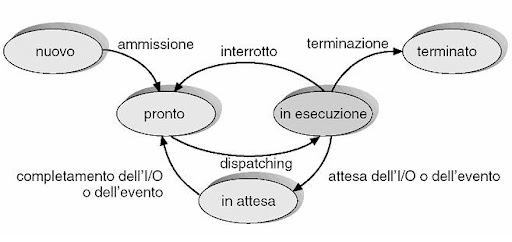
\includegraphics[width=0.5\textwidth]{immagini/processo a 5 stati}
    \caption{Modello dei processi a 5 stati}
\end{figure}
Cosa c' é dietro a blocked ? il processo é in attesa di un evento, es. I/O, il processo é sospeso e il sistema operativo
si occupa di far partire un altro processo, quando l'evento é completato il processo torna in ready. il dispatcher per cui
non metterá mai un processo blocked in esecuzione.
Con 5 stati abbiamo bisogno quindi 2 code di processi:
\begin{itemize}
    \item Ready Queue: contiene i processi pronti per essere eseguiti
    \item Blocked Queue: contiene i processi in attesa di un evento
\end{itemize}
I sistemi operativi hanno piú di una coda di eventi che contiene gli eventi che devono essere completati, quando un evento é completato
il processo torna in ready
\begin{figure}
    \centering
    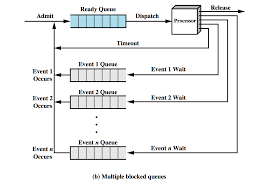
\includegraphics[width=0.5\textwidth]{immagini/5StatiCode2}
    \caption{Diagramma delle 2 code di processi}
\end{figure}
\subsection{Processi Sospesi}
Esiste la possibilitá di avere dei processi sospesi, questo é dovuto quando molti processi sono in attesa di un evento,
quindi fino a che sono bloccati non possono essere eseguiti, quindi vengono spostati dalla RAM al disco, in questo modo
si libera spazio in RAM, quando l'evento é completato il processo viene spostato dalla memoria secondaria alla RAM,
questo cambiamento aggiunge 2 stati ai 5 precedenti:
\begin{itemize}
    \item Ready Suspended: il processo é pronto per essere eseguito ma é sospeso
    \item Blocked Suspended: il processo é in attesa di un evento ma é sospeso
\end{itemize}
\begin{figure}
    \centering
    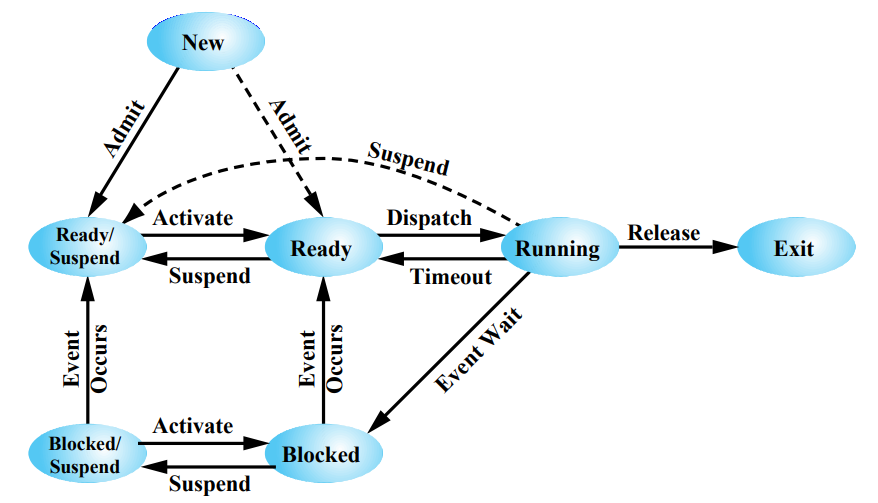
\includegraphics[width=0.5\textwidth]{immagini/7State}
    \caption{Modello dei processi a 7 stati}
\end{figure}
I motivi per sospendere un processo sono:
\begin{itemize}
    \item Swapping: il processo é spostato dalla RAM al disco
    \item Interno al OS : Il sistema sospetta che il processo stia causando problemi
    \item Periodicitá: il processo viene eseguito solo periodicamente
    \item Richiesta del processo padre : il processo padre puó richiedere di sospendere un processo figlio
\end{itemize}
\subsection{Strutture di controllo del OS}
Il sistema operativo é l'entitá che si occupa di gestire le risorse da parte dei processi,
per fare ció esso deve conoscere lo stato di ogni processo, per compiere questa operazione il sistema operativo
crea 1 o piú tabelle
\begin{figure}
    \centering
    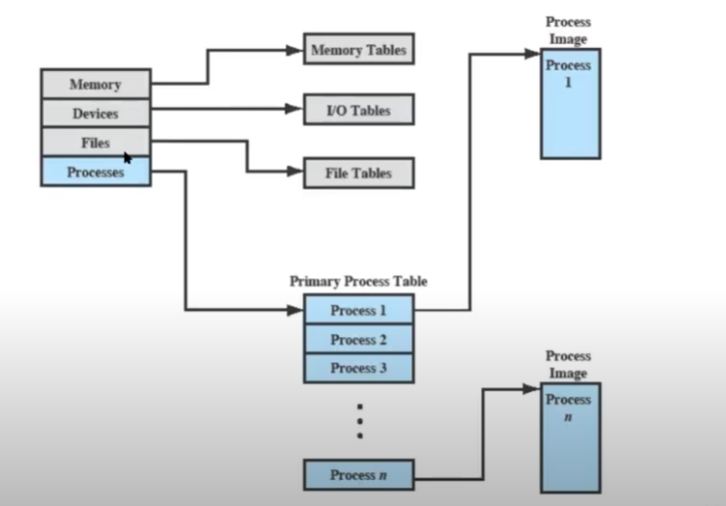
\includegraphics[width=0.5\textwidth]{immagini/ControlTable}
    \caption{Strutture di controllo del OS}
\end{figure}
per ciascuna delle risorse esistono tabelle per gestire la memoria, i file, i dispositivi di I/O e i processi
tutte queste tabelle si trovano nella zona di memoria riservata al kernel
\subsubsection{Memory Table}
Le tabelle di memoria sono usate per gestire sia la memoria principale che quella secondaria(quella secondaria serve per la memoria virtuale),
le tabelle di memoria contengono informazioni su:
\begin{itemize}
    \item allocazione di memoria principale da parte dei processi
    \item allocazione di memoria secondaria da parte dei processi
    \item attributi di protezione per l'accesso a zone di memoria
    \item informazioni per gestire la memoria virtuale
\end{itemize}
\subsubsection{Tabelle per l'I/O}
Le tabelle per l'I/O contengono informazioni su:
\begin{itemize}
    \item se il dispositivo é disponibile o giá assegnato
    \item lo stato dell'operazione di I/O
    \item la locazione in memoria principale usata come sorgente o destinazione dell'operazione di I/O
\end{itemize}
\subsubsection{File Table}
Le tabelle per i file contengono informazioni su:
\begin{itemize}
    \item Esistenza di un file
    \item Locazioni in memoria secondaria
    \item Stato corrente
    \item Altri attributi
\end{itemize}
\subsubsection{Process Table}
Per gestire i processi il sistema operativo usa una tabella di processi, che contiene informazioni su:
\begin{itemize}
    \item Stato del processo
    \item identificatore del processo
    \item locazione in memoria
\end{itemize}
Blocco di controllo dell'processo (PCB) é un blocco di informazioni che contiene tutte le informazioni necessarie per gestire un processo
\newline
Si dice \textbf{process image} l'insieme di programma sorgente,dati,stack delle chiamate e PCB, eseguire un'istruzione cambia l'immagine
, unica possiblie eccezzione é l'istruzione di jump all'istruzione stessa.
\subsection{Attributi di un processo}
Le informazioni in ciascun bloocco di controllo del processo possono essere raccolte in 3 gruppi:
\begin{itemize}
    \item Identificazione
    \item Stato
    \item Controllo
\end{itemize}
\subsubsection{Come si Identifica un processo}
ad ogni processo é assegnato un identificatore unico, che é un intero positivo, Molte tabelle del OS usano PID
per realizzare collegamenti tra le varie tabelle.
\subsubsection{Stato del processore}
Da non confondere con lo stato del processo, é dato dai contenuti dei registri del processore stesso:
\begin{itemize}
    \item registri visibili all'utente
    \item registri di controllo e di stato
    \item puntatori allo stack
    \item PSW(Program Status Word) : la program status word contiene informazioni sullo stato del processo
    \end{itemize}
\subsubsection{Control Block del Processo}
Per Ricapitolare il PCB contiene:
\begin{itemize}
    \item Contiene informazioni di cui l'OS ha bisogno per coordinare processi attivi
    \item Identificatori : PID, PPID (parent process ID) oppure dell'utente che lo ha eseguito
    \item Informazioni sullo stato del processore : registri utente, program counter, stack pointer e registri di stato
    \item Informazioni per il controllo del processo : priorità, stato del processo, informazioni di scheduling, l'evento d'attender per essere ready
    \item Supporto per strutture dati: puntatori ad altri processi, per fare code di processi o liste di processi
    \item Comunicazione tra processi: informazioni per la comunicazione tra processi flag,segnali,messaggi
    \item Permessi Speciali: permessi speciali per l'accesso a risorse
    \item Gestione della memoria: puntatori ad aree di memoria
    \item Gestione delle Risorse : file aperti, ecc.
\end{itemize}
\subsection{Processi e Memoria virtuale}
Se ci sono n processi attivi, ci sono n PCB, e sono conservati nella ram conservati nella zona del kernel, tutto il
resto é conservato nella memoria virtuale, una parte della memoria virtuale puó essere condivisa tra i processi mentre
normalmente un processo non puó accedere alla memoria di un altro processo é peró possibile
condividere la memoria se chi ha scritto il programma lo ha previsto, es. condividere una variabile tra 2 processi.
Tutto questo fa si che il control block sia una delle strutture dati piú importanti del sistema operativo perché definisce lo stato dell'OS stesso,
Richiede inoltre Protezione, una funzione scritta male potrebbe danneggiare il blocco.
\subsection{Modalita di esecuzione}
La maggior parte dei processori supporta almeno due modalitá di esecuzione:
\begin{itemize}
    \item Modalitá utente: molte operazioni non sono permesse
    \item Modalitá kernel : pieno controllo del processore ad esempio si possono eseguire istruzione macchina
\end{itemize}
\subsubsection{Kernel Mode}
Il kernel mode é la modalitá di esecuzione in cui il sistema operativo ha il controllo completo del processore,
si possono gestire i processi (tramite PCB)
\begin{itemize}
    \item creazione e terminazione di processi
    \item pianificazione di lungo,messo e corto termine(scheduling e dispatching)
    \item avvicendamento dei processi(switching)
    \item sincronizzazione e comunicazione tra processi
\end{itemize}
si puó gestire la memoria principale:
\begin{itemize}
    \item allocazione di spazio
    \item gestione della memoria virtuale
\end{itemize}
si puó gestire l'I/O:
\begin{itemize}
    \item gestione dei buffer e delle cache per l'I/O
    \item assegnazione risorse I/O ai processi
\end{itemize}
Funzioni Supporto: Gestione interrupt/eccezzioni,accounting,monitoraggio
\subsubsection{Da UserMode a KernelMode}
Esite quindi la necessita di passare da user mode a kernel mode, esempio: un processo vuole fare una operazione di I/O,
deve chiedere il permesso al sistema operativo, di passare in kernel mode, per poi tornare in user mode.
Ogni processo inizia sempre in user mode, se viene fatta una richiesta che necessita della kernel mode come una system call
il processo passa in kernel mode, il sistema operativo esegue la system call e poi torna in user mode, l'ultima istruzione
dell'interrupt handler é una istruzione di ritorno che fa tornare il processo in user mode.
esistono quindi 3 casi in cui si passa in kernel mode:
\begin{itemize}
    \item Codice eseguito per conto dello stesso processo interrotto, che lo ha esplicitamente voluto
    \item Codice eseguito per conto dello stesso processo interrotto, che non lo ha esplicitamente voluto
    \item Codice eseguito per conto di un altro processo
\end{itemize}
Esempio di system call sui pentium:
\begin{enumerate}
    \item prepara gli argomenti della chiamata nei registri, tra tali argomenti c'é un numero che identifica la system call
    \item esegue lístruzione int 0x80, che appunto solleva un interrupt(in realtá una eccezzione)
    \end{enumerate}
Anche creare un nuovo processo é una system call : l'handler di questa system call verrá ovviamente eseguito in modalitá kernel,puó quindi modificare la lista dei PCB
\subsection{Creazione del processo}
per creare un processo il sistema operativo deve:
\begin{itemize}
    \item Assegnargli un PID Unico
    \item Allocargli spazio in memoria principale
    \item Inizializzare il PCB
    \item Inserire il processo nella giusta coda
    \item Creare o espandere strutture dati
\end{itemize}
\subsection{Switching tra processi}
Lo switching tra processi é il passaggio da un processo all'altro, ovver per qualche motivo l'attuale processo non deve piú usare
il processore che concesso ad un altro processo.
\subsubsection{Quando effettuare lo switching}
Lo switching tra processi puó avvenire per diversi motivi:
\begin{itemize}
    \item interruzzione : Cause esterna all'esecuzione dell'istruzione corrente Uso Reazione a un evento esterno asincrono, include i quanti di tempo per lo scheduler
    \item Eccezzione: Associata all'esecuzione dell'istruzione, gestione di un errore sincrono
    \item Chiamata al OS : Richiesta esplicita, chiamata a funzione di sistema
\end{itemize}
\subsubsection{Passaggi per lo switching}
\begin{enumerate}
    \item Salvare il contesto del programma (registri e PC) salvati nel PCB
    \item Aggiornare il process control block, attualmente in running
    \item Spsotare il PCB nella coda appropriata : ready,blocked;ready/suspended
    \item Scelgiere un nuovo processo da eseguire
    \item Aggiornare il process control block del processo selezionato
    \item Aggiornare le strutture dati per la gestione della memoria
    \item Ripristinare il contesto del processo selezionato
\end{enumerate}
\subsubsection{Il Sistema operativo é un processo}
Il sistema operativo é un insieme di programmi, ed é eseguito dal processore come ogni altro programma, semplicemente
lascia che altri programmi vadano in esecuzione, per poi riprendere il controllo tramite interrupt, quindi se é un processo lui stesso
deve essere gestito...
esistono quinndi 3 modi per gestire il sistema operativo:
\begin{itemize}
    \item kernel separato : il sistema operativo é un processo separato
    \item kernel unico : il sistema operativo é un processo come gli altri
    \item Sistemi ibridi : il sistema operativo é un processo separato, ma esiste un kernel unico
\end{itemize}
\subsubsubsection{Kernel non é un processo}
il kernel é eseguito al di fuori dei processi, il concetto di processo si applica solo ai processi utente, il kernel é eseguito
\subsubsubsection{Esecuzione all'interno dei processi utenti}
Il SO viene eseguito nel contesto di un processo utente, non c'é bisogno di un process switch per eseguire una funzione del sistema operativo,
sole del mode switch, Comunque , stack delle chiamate separato, process switch solo,eventualmente, per passare il controllo ad un altro processo
\subsubsubsection{Sistema Basato su processi}
il sistema operativo é un insieme di processi, ogni processo é un modulo del sistema operativo, ogni processo é un modulo del sistema operativo,
ogni processo partecipa alla competizione per il processore, lo switch peró non é un processo
\subsubsection{Esempio in Linux}
In linux ci sono peró anche dei processi di sistema, che partecipano alla normale competizione per il processore, senza essere invocati esplicitamente,
sono operazioni tipiche del sistema operativo, es. gestione della memoria, gestione dei dispositivi di I/O
\begin{figure}
    \centering
    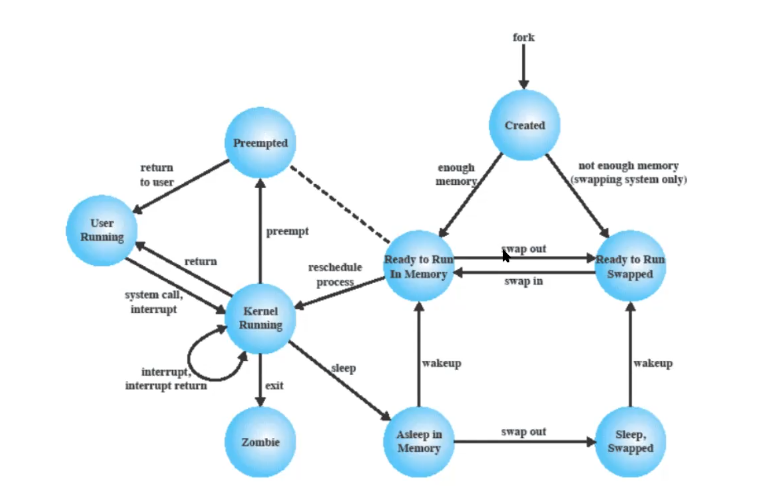
\includegraphics[width=0.75\textwidth]{immagini/transizioneTraStatiDeiProcessi}
    \caption{Diagramma stati Unix}
\end{figure}
\subsubsection{Stati in Unix}
Con l'istruzione fork() si crea un processo figlio,
una volta che il processo é stato creato, abbiamo 2 possibili stati Run in memory oppure Run in swapped(Memoria Virtuale)
i due stati sono intercambiabili ovvero posso spostare il processo dalla memoria principale alla memoria virtuale e viceversa
anche lo stato di sospensione puó avvenire in memoria o in memoria virtuale. Quando il processo in running si trova in user mode
, quando vengono effettuate delle system call il processo passa in kernel mode, quando siamo in kernel mode c'é la possibilitá di
effettuare la preemption, ovvero sospendere il processo per farne eseguire un altro, il processo puó essere sospeso per un interrupt
, nello stato di preemption si prende in considerazione l'idea di non continuare l'esecuzione, quando un processo finisce va
nello stato zombie (Tipico dei sistemi Unix), quello che succede é che ci si aspetta che il processo padre soppravviva al figlio
e fino a che il processo figlio non comunica al padre che ha terminato, il processo figlio rimane nello stato zombie, l' unica cosa
che rimane é il PCB, quando il processo padre comunica al sistema operativo che il processo figlio é terminato, il processo figlio.
\subsubsection{Transizione tra processi}
non é interrompibile quando siamo in kernel mode quindi non va bene per sistemi real time
\subsection{Immagine del processo in Unix}
Un insieme di strutture dati forniscono al sistema operativo le informazioni necessarie per gestire un processo
\begin{itemize}
    \item User Area : contiene il codice, i dati e lo stack del processo
    \begin{enumerate}
        \item \textbf{Codice}: linguaggio macchina
        \item \textbf{Dati}: variabili globali e locali
        \item \textbf{Stack}: contiene le informazioni necessarie per gestire le chiamate a funzione
        \item \textbf{Memoria Condivisa}: usata per la comunicazione tra processi (deve essere esplicitamente richiesta)
    \end{enumerate}
    \item Registro : contiene i registri del processore
    \begin{enumerate}
        \item \textbf{Program Counter}: contiene l'indirizzo dell'istruzione corrente
        \item \textbf{Stack Pointer}: contiene l'indirizzo della cima dello stack
        \item \textbf{Registri Generali}: contengono i dati temporanei
    \end{enumerate}
    \item sistema : contiene le informazioni necessarie per la gestione del processo a livello di memoria
    \begin{enumerate}
        \item \textbf{Process Table Entry}: puntatore alla tabella di tutti i processi, dove individua quello corrente
        \item \textbf{U Area}: informazioni per il controllo dell'processo, informazioni addizzionali per quando il kernel viene eseguito da questo processo
        \item \textbf{Per process region table}: definisce il mapping tra indirizzi logici e fisici (Page Table), inoltre indica se per questo processo tali indirizzi sono in lettura, scrittura o esecuzione
        \item \textbf{Kernel Stack}: Stack delle chiamate, separato da quello utente, usato per le funzioni da eseguire in modalitá sistema (kernel mode)
    \end{enumerate}
\end{itemize}
\begin{table}[H]
    \raggedright
    \begin{tabular}{|c|p{10cm}|}
        \hline
        Process Status & Current State \\
        \hline
        Pointers & puntatori alle zone del processo\\
        \hline
        Process Size & quanto é grande l' immagine del processo (il PCB ha una grandezza predefinita) \\
        \hline
        User Identifier & Identificatore dell'utente che ha lanciato il processo, c'é una differenza tra \textbf{Real User ID} e \textbf{ effective user ID}  \\
        \hline
        Process ID & Identificatore del processo \\
        \hline
        Event Descriptor & Motivazioni per il quale il processo é bloccato \\
        \hline
        Priority & Prioritá del processo \\
        \hline
        Signal State & Stato dei segnali \\
        \hline
        Timers & Include il tempo di esecuzione del processo, l'utilizzo delle risorse del kernel, timer usati per mandare segnali di allarme ad un processo \\
        \hline
        P_Links & Puntatori per le code di processi(LinkedList), \\
        \hline
        Memory Status & Indicazioni se la memoria é in memoria principale o secondaria, indica anche se il processo se puó essere spostato \\
        \hline
    \end{tabular}
    \caption{Process Table entry}
    \label{tab:esempio}
\end{table}
    \section{I Thread}
Ci sono alcune applicazioni che richiedono la gestione in parallelo, ovvero quando viene programmata un'applicazione
viene suddivisa in piú parti, quindi l'applicazione rimane un singolo processo, ma che al suo interno esegue
piú computazioni in parallelo, quindi possiamo dire che un processo puó essere composto da piú thread.
In questo caso é compito del programmatore occuparsi della sincronizzazione tra i thread, il sistema operativo
si occupa di gestire i processi, mentre il programmatore si occupa di gestire i thread.
Diversi thread condividono molte risorse, del processo, non condividono lo stack delle chiamate ed anche il processore,
condividono invece memoria(Stack Esclusi), files, dispositivi di I/O, ecc.
Teoricamente si puó dire che il processo incorpori gestione delle risorse e scheduling
\begin{figure}[H]
    \centering
    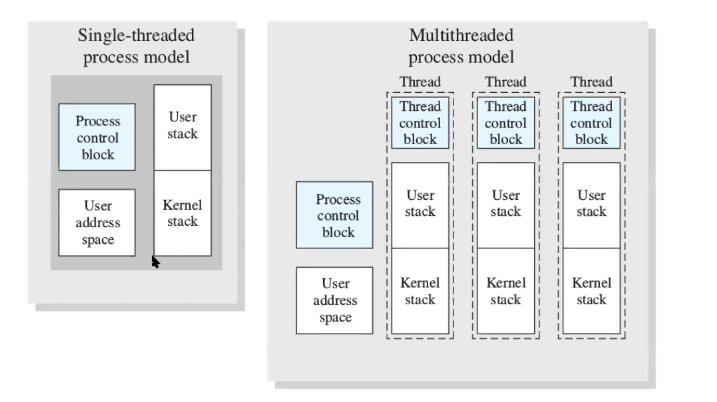
\includegraphics[width=0.5\textwidth]{immagini/thread1}
    \caption{Thread}
\end{figure}
Se sono su un sistema operativo Single Threaded, il sistema operativo non supporta il multithreading, ho l'immagine del processo
ed il PCB, se il sistema operativo supporta il multithreading, ho l'immagine del processo, il PCB e il TCB(Thread Control Block),
dove Il TCB gestisce solo la parte dello scheduling
\subsection{Perché introdurre i thread}
Creare un thread é semplice/efficiente, la creazione la terminazione, fare lo switching e farli comunicare,
quindi ogni processo viene creato con un thread, dopo il programmatore puo' creare altri thread con il comando spawn()
, esistono chiamate di sistema per bloccare un thread, sbloccare un thread, terminare un thread.
\subsection{ULT e KLT}
Esistono 2 tipi di thread:
\begin{itemize}
    \item ULT(User Level Thread): A livello di sistema operativo i thread non esistono, oppurtune librerie si occupano di gestire il thread
    \item KLT(Kernel Level Thread): Il sistema operativo supporta i thread, quindi il sistema operativo é a conoscenza dei thread
    \item
\end{itemize}
\begin{figure}[H]
    \centering
    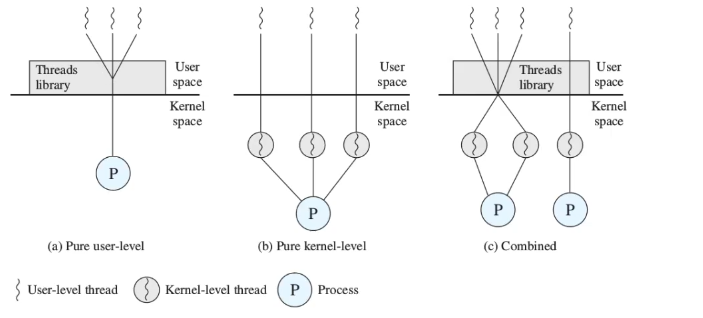
\includegraphics[width=0.5\textwidth]{immagini/ULTeKLT}
    \caption{ULT e KLT}
\end{figure}
perché usare ULT:
\begin{itemize}
    \item Sono piú veloci da creare e gestire (Non serve fare il mode swithcing)
    \item Si puó avere una politica di scheduling per ogni processo
    \item Permettono di usare i thread anche sui sistemi operativi che non li offrono nativamente
\end{itemize}
perché NON usare ULT:
\begin{itemize}
    \item Se un thread si deve bloccare, si bloccano tuitti i thread del processo, a meno che il blocco non sia chiamato
    dalla chiamata di block, al contrario con i KLT solo il thread che si blocca viene bloccato
    \item Se ci sono piú processori o piú core, i thread non possono essere eseguiti in parallelo perché il sistema operativo
    non é a conoscenza dei thread
\end{itemize}
\subsection{Processi e Thread in Linux}

I thread sono spesso associati al termine Light Weight Processes o LWP. Questo termine risale ai tempi in cui Linux supportava i thread solo a livello utente. Ciò significa che anche un'applicazione multithread era vista dal kernel come un singolo processo. Questo creava grandi sfide per la libreria che gestiva questi thread a livello utente, poiché doveva garantire che l'esecuzione di un thread non fosse ostacolata se un altro thread emetteva una chiamata bloccante.

Successivamente l'implementazione è cambiata, e ai processi sono stati collegati singoli thread, in modo che fosse il kernel a gestirli. Tuttavia, come discusso in precedenza, il kernel Linux non li vede come thread: ogni thread è trattato come un processo all'interno del kernel. Questi processi sono conosciuti come processi leggeri o light weight processes.

La principale differenza tra un processo leggero (LWP) e un processo normale è che gli LWP condividono lo stesso spazio di indirizzamento e altre risorse come i file aperti. Poiché alcune risorse sono condivise, questi processi vengono considerati più "leggeri" rispetto agli altri processi normali, da cui il nome di processi leggeri.

Quindi, in sostanza, possiamo dire che thread e processi leggeri sono la stessa cosa. È solo che thread è un termine usato a livello utente, mentre light weight process è un termine utilizzato a livello di kernel.


Nel kernel, ogni thread ha il proprio ID, chiamato PID (anche se forse avrebbe più senso chiamarlo TID), e ha anche un TGID (Thread Group ID) che corrisponde al PID del thread che ha avviato l'intero processo.

Semplificando, quando viene creato un nuovo processo, appare come un thread in cui sia il PID che il TGID sono lo stesso nuovo numero.

Quando un thread avvia un altro thread, il thread avviato ottiene il proprio PID (in modo che lo scheduler possa programmarlo indipendentemente), ma eredita il TGID dal thread che lo ha creato.

In questo modo, il kernel può programmare i thread indipendentemente dal processo a cui appartengono, mentre i processi (gli ID del gruppo di thread, o TGID) vengono mostrati agli utenti.

Per ogni thread, esiste quindi un PCB per ogni thread, questo crea un piccolo overhead perché esiste una duplicazione di alcune informazioni(puntatori)
\subsection{Gli stati dei processi in Linux}
Linux ha 5 stati per i processi, linux non distingue tra ready e running, divide peró in due stati blocked,
\begin{itemize}
    \item Task Running: il processo é in esecuzione sulla CPU
    \item Blocked:
    \begin{enumerate}
        \item Task Interruptible: il processo é in attesa di un evento, ma puó essere interrotto
        \item Task Uninterruptible: il processo é in attesa di un evento, ma non puó essere interrotto
        \item Task Stopped: il processo é stato fermato
        \item Task Traced: il processo é tracciato
    \end{enumerate}
    \item EXIT Zombie: il processo é terminato, ma il processo padre non ha ancora comunicato al sistema operativo
    \end{itemize}
\subsection{Segnali ed interrupt in Linux}
Non bisogna confondere i segnali con gli interrupt, I segnali possono essere inviati da un processo ad un altro processo,
quello che succede che il campo del PCB viene aggiornato con il segnale che é stato inviato, quando il processo
viene schedulato, il kernel controlla se ci sono segnali da gestire se si esegue la funzione di gestione del segnale,
alcuni signa handlers possono essere sovrascritti dal programmatore, alcuni segnali hanno l'handler non sovrascrivibile,
in ogni caso sono eseguiti in user mode, mentre gli interrupt sono eseguiti in kernel mode.
    
    \section{Scheduling}
Un sistema operativo deve allocare risorse tra i processi, tra le risorse quella piú ovvia é il processore, l' uso del
    processore é detto scheduling, la metodologia che gestisce l'uso del processore é detta politica di scheduling,
    lo scopo dello scheduling é assegnare ad ogni processore qualcosa de eseguire, bisogna quindi che lo scheduling
    sia il piú efficiente possibile, tenendo conto di vari aspetti:
    \begin{itemize}
        \item tempo di risposta (Tendo a minimizzare)
        \item throughput (Tendo a massimizzare)
        \item efficienza del processore (Tendo a massimizzare)
    \end{itemize}
    altri obbiettivi dello scheduling é non fare favoritismi tra i processi, tuttavia nei moderni sistemi operativi
    esiste la priorità dei processi, quindi alcuni processi vengono privilegiati rispetto altri, inoltre lo scheduling
    deve evitare lo starvation, ovvero che un processo non venga mai eseguito, noon lasciare mai il processore inattivo,
    avere un overhead basso (il tempo per fare lo scheduling deve essere il piú basso possibile),
    \subsection{Tipi di scheduling}
    \begin{itemize}
        \item Long-term scheduling: decide quali processi devono essere caricati in memoria
        \item Medium-term scheduling: decide quali processi devono essere spostati dalla memoria principale alla memoria secondaria
        \item Short-term scheduling: decide quale processo deve essere eseguito sulla CPU
        \item I/O scheduling: decide quale processo deve essere eseguito sul dispositivo di I/O
    \end{itemize}
    \begin{figure}[H]
        \centering
        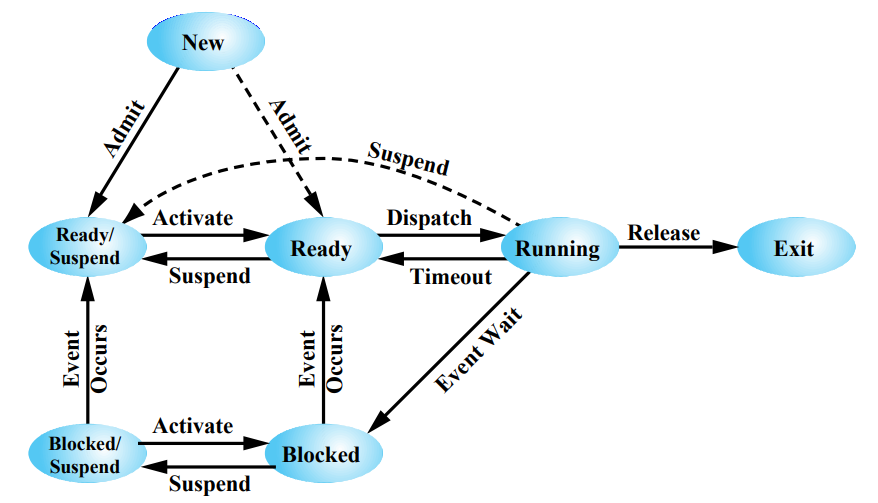
\includegraphics[width=0.5\textwidth]{immagini/7State}
        \caption{Tipi di scheduling}
    \end{figure}
    abbiamo visto che si di ready che di blocked ci sono le versioni suspended (sono in memoria secondaria), molte
    delle transizioni sono dovute allo scheduler, quello che decide se un processo appena creato Ready o Ready Suspended
    é il long-term scheduler, il medium-term decide tra le versioni suspended e non suspended, il short-term scheduler
    decide se un processo é Ready o Running, il I/O scheduler decide se un processo é Blocked o Ready
    \begin{figure}[H]
        \centering
        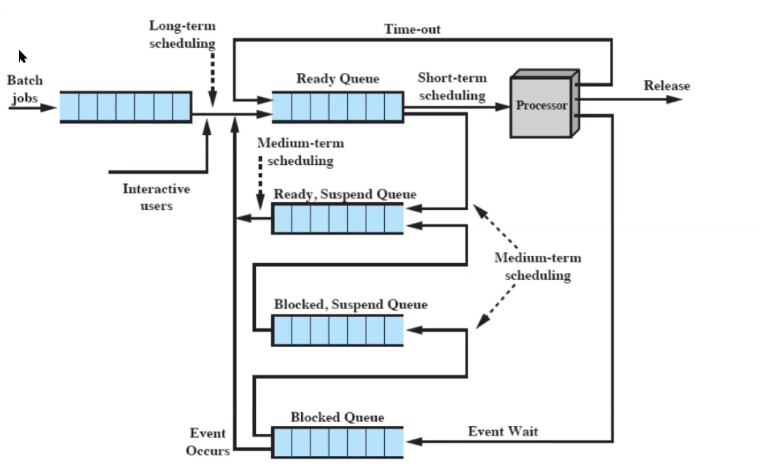
\includegraphics[width=0.5\textwidth]{immagini/implementazioneScheduling}
        \caption{Tipi di scheduling}
    \end{figure}
    lo scheduling fa una distinzione tra processi interattivi e processi batch, i processi in batch hanno una coda, mentre
    quelli interattivi cercano direttaqmente di essere eseguiti, Il long-term come detto sopra decide se i processi sono
    messi in ready o ready suspended, il medium term scheduler decide se un processo é messo in ready o ready suspended
    oppure blocked o blocked suspended e viceversa, il short term scheduler decide se un processo é messo in running o blocked
    \subsection{Long-term scheduling}
    Decidide quali programmi sono ammessi nel sistema, spesso segue una logica FIFO (First In First Out),
    spesso é un FIFO "Corretto, tenendo conto di criteri come la priorità, il tempo di esecuzione, ecc.

    Inoltre controlla il grado di multiprogrammazione, ovvero il numero di processi che possono essere eseguiti
    contemporaneamente, il grado di multiprogrammazione é il numero di processi che possono essere eseguiti
    contemporaneamente,

    Piú processi ci sono, piú é piccola la percentuale di tempo per cui ogni processo viene eseguito.

    Le strategie di scheduling sono:
    \begin{itemize}
        \item i lavori batch vengono accodati e il LTS li prende man mano che il processore é libero
        \item I lavori interattivi vengono ammessi fino a saturazione del sistema
        \item Se si sa quali processi sono I/O bound e quali sono CPU bound, si possono fare scelte migliori facendo un giusto mix tra due tipi
        \item Se si sa quali processi fanno richieste a quali dispositivi, di I/O, fare in modo di bilanciare le richieste
    \end{itemize}
    Il Long-term scheduler puó essere chiamato anche quando non ci sono nuovi processi, ad esempio quando termina un processo oppure
    quando un processo é idle da troppo tempo.

    \subsection{Medium-term scheduling}
    Il medium-term scheduler decide se bisogna fare degli aggiustamenti tra RAM e Disco, il motivo principale é quello di gestire
    la multiprogrammazzione, se terminano 10 processi ad esempio, il medium term scheduler decide quali processi ready
    presenti in memoria secondaria devono essere spostati in memoria principale, il medium term scheduler é chiamato anche
    \subsection{short-term scheduling}
    Il short-term scheduler é chiamato anche dispatcher, decide quale processo deve essere eseguito sulla CPU,
    ed é quello eseguito piú frequentemente.viene invocato in seguito a:
    \begin{itemize}
        \item interruzzioni di clock
        \item interruzzioni di I/O
        \item chiama di sistema
        \item segnali
    \end{itemize}

    Lo scopo dello short-term scheduler é quello di allocare tempo di esucozione tra i processori, per ottimizzare
    il comportamento dell'intero sistema, per valutare quindi una politica di scheduling bisogna valutare:
    \begin{itemize}
        \item Utente: tempo di risposta, tempo di esecuzione
        \item Sistema: throughput, efficienza del processore
    \end{itemize}
    L' altra categoria é quella se sono criteri se sono criteri prestazionali (quantitativi) oppure quelli non
    prestazionali (qualitativi) che sono piú difficili da misurare.
    \subsubsection{Criteri Utente}
    Prestazionali :
        \begin{itemize}
        \item   \textbf{Turnaround time}: tempo tra la creazione e la terminazione di un processo
        \item  \textbf{Tempo di risposta}: tempo tra la creazione e la prima risposta
        \item  \textbf{Deadline}: tempo entro il quale un processo deve essere completato
    \end{itemize}
    Non Prestazionali:
    \begin{itemize}
        \item \textbf{Predictability}: quanto é prevedibile il tempo di esecuzione
    \end{itemize}
    \subsubsection{Criteri di sistema}
    Prestazionali:
    \begin{itemize}
        \item \textbf{Throughput}: numero di processi completati in un certo intervallo di tempo
        \item \textbf{Efficienza del processore}: percentuale di tempo in cui il processore é utilizzato
    \end{itemize}
    Non Prestazionali:
    \begin{itemize}
        \item \textbf{Equità}: tutti i processi devono avere la stessa possibilitá di essere eseguiti
        \item \textbf{Enforces priorities}: i processi con priorità piú alta devono essere eseguiti prima
        \item \textbf{Balancing resources}: bilanciare l'uso delle risorse
        \end{itemize}
    \subsection{Turnaround time}
    Il turnaround time é il tempo tra la creazione e la terminazione di un processo, comprende i vari tempi di attesa (I/O, CPU, ecc.)
    si usa spesso per processi non interattivi.
    \subsection{Tempo di risposta}
    Il tempo di risposta é il tempo tra la creazione e la prima risposta, é importante per i processi interattivi (es. un utente che clicca su un bottone)
    lo scheduler in questo caso ha un duplice obbiettivo per lo scheduler: minimizzare il tempo di risposta medio
    e massimizzare il numero di utenti che hanno un risposta veloce.
    \subsection{Deadline}
    La deadline é il tempo entro il quale un processo deve essere completato, é importante per i processi real-time,
    un buon dispatcher deve massimizzare il numero di scadenze rispettate, per quanto riguarda invece la Predictability
    se lancio tante volte lo stesso processo, il tempo di esecuzione deve essere sempre lo stesso, altrimenti il
    dispatcher non é prevedibile.
    \subsection{Throughput}
    Il throughput é il numero di processi completati in un certo intervallo di tempo, ovviamente l' obbietti é massimizzare
    il throughput, é una misura di quanto lavoro viene effettuato.
    \subsection{Utilizzo del processore}
    L' utilizzo del processore é la percentuale di tempo in cui il processore é utilizzato, ovviamente l' obbiettivo é massimizzare
    l' utilizzo del processore, quindi il processore non deve mai essere inattivo, questo é un criterio molto costosi condivisi
    tra piú utenti.
    \subsection{Bilanciamento delle risorse}
    Lo scheduler deve bilanciare l'uso delle risorse, ad esempio se un processo é CPU bound, non ha senso assegnargli un
    tempo di I/O, quindi lo scheduler deve bilanciare l'uso delle risorse, quindi processi che utilizzano meno le risorse attualmente
    piú usate devono essere favoriti.
    \subsection{Fairness e Priorità}
    La fairness é il concetto che tutti i processi devono avere la stessa possibilitá di essere eseguiti, per cui non sono
    presenti favoritismi, a meno che non ci siano priorità, in questo caso i processi con priorità piú alta devono essere eseguiti
    prima, inoltre questo causera la creazioni di code di processi, quindi lo scheduler deve essere in grado di gestire le code
    di processi.
    \subsection{Prioritá e Starvation}
    La prioritá ha un problema, ovvero che puó indurre starvation, esempio: se un processo ha una bassa priorità, potrebbe
    non essere mai eseguito, quindi lo scheduler deve evitare lo starvation, ovvero che un processo non venga mai eseguito,
    per evitare lo starvation si puó usare la politica di aging, ovvero aumentare la priorità di un processo che non viene mai eseguito.
    \subsection{Politiche di scheduling}
    \begin{figure}[H]
        \centering
        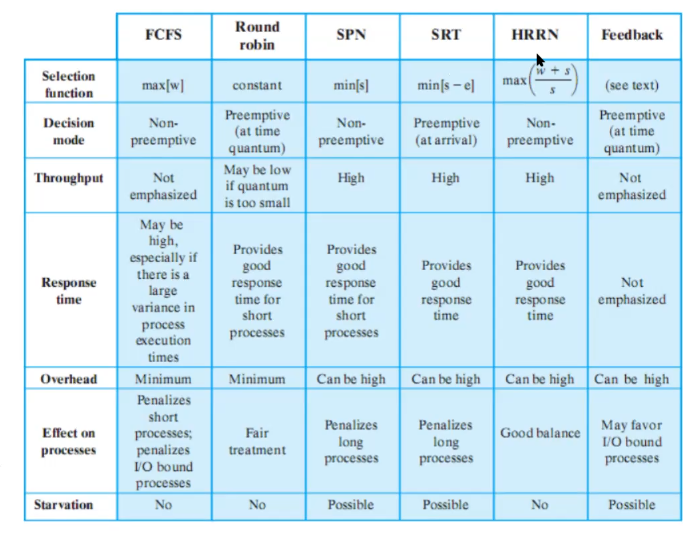
\includegraphics[width=1\textwidth]{immagini/PoliticheDiScheduling}
        \caption{Politiche di scheduling}
    \end{figure}
    Raramente si usa una sola politica di scheduling, si usano piú politiche di scheduling, inoltre non si
    utilizzano gli algoritmi di scheduling implementate, ma revisioni di esse.
    \subsection{Selection Function}
    La selection function é quella che sceglie effetivamente quale processo deve essere eseguito,
    la scelta viene fatta in base a vari criteri:
    \begin{itemize}
        \item w = tempo di attesa
        \item e = tempo trascorso in esecuzione
        \item s = tempo totale richiesto (stimato), incluso quello giá servito (e)
    \end{itemize}
    \subsection{Decision Mode}
    Specifica in quali istanti di tempo la funzione di selezione viene invocata, ci sono 2 possibili modi:
    \begin{itemize}
        \item Non pre-emptive: la funzione di selezione viene invocata solo quando il processo in esecuzione termina
        \item Pre-emptive: la funzione di selezione viene invocata ad intervalli regolari
    \end{itemize}
    \subsubsection{Pre-emptive - Non pre-emptive}
    Non pre-emptive: se un processo é in esecuzione, allora arriva o fino a terminazione of fino ad un I/O, non gli tolgo il processore

    Pre-emptive: Il sistema operativo puó interrompere un processo in esecuzione per eseguire un altro processo, in questo caso il processo
    passera da running a ready, la preemption di un processo puó avvenire o pre l'arrivo di nuovi processi (appena creati) o per un interrupt di I/O,
    oppure per interrupt di clock, quest'ultimo é periodico per evitare che alcuni processi monopolizzino il processore.
    \subsection{ESEMPIO}
    Scenario Comune :
    \begin{table}[H]
        \raggedright
        \begin{tabular}{|c|c|c|}
            \hline
            \textbf{Processo} & \textbf{Tempo di arrivo} & \textbf{Tempo di esecuzione} \\
            \hline
            A & 0 & 3   \\
            \hline
            B & 2 & 6 \\
            \hline
            C & 4 & 4  \\
            \hline
            D & 6 & 5  \\
            \hline
            E & 8 & 2  \\
            \hline
        \end{tabular}
    \end{table}
    \subsection{First Come First Served}
    Tutti i processi sono aggiunti alla coda ready, é non pre-emptive, quando il processo ha finito di essere eseguito, si passa
    al processo che ha aspettato di piú nella coda.
    \begin{figure}[H]
        \centering
        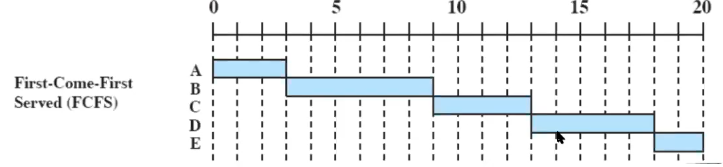
\includegraphics[width=0.75\textwidth]{immagini/FCFS}
        \caption{First Come First Served}
    \end{figure}
    L' algoritmo é molto semplice, é anche molto equo, dal punto di vista del sistema operativo, un processo corto
    deve aspettare che altri processi terminino, favorisce i processi CPU bound, per cui degenera perché un processo 
    monopolizza il processore.
    \subsection{Round Robin}
        \begin{table}[H]
        \raggedright
        \begin{tabular}{|c|c|c|}
            \hline
            \textbf{Processo} & \textbf{Tempo di arrivo} & \textbf{Tempo di esecuzione} \\
            \hline
            A & 0 & 3   \\
            \hline
            B & 2 & 6 \\
            \hline
            C & 4 & 4  \\
            \hline
            D & 6 & 5  \\
            \hline
            E & 8 & 2  \\
            \hline
        \end{tabular}
    \end{table}
    Il round robin usa la preemption, basandosi su un clock, Talvolta chiamato time slicing, perché ogni processo
    ha una fetta di tempo, é un algoritmo di scheduling per processi interattivi.
    \begin{figure}[H]
        \centering
        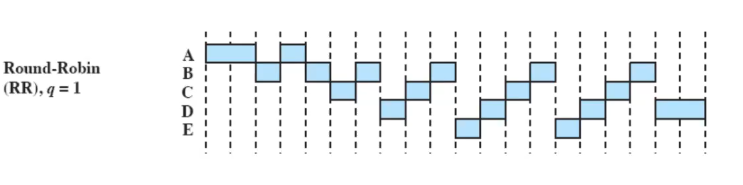
\includegraphics[width=0.75\textwidth]{immagini/RoundRobin}
        \caption{Round Robin}
    \end{figure}
    in questo caso il processo E finisce prima rispetto all'algoritmo FCFS, nel
    caso ci sia una coda si utilizza una politica FIFO, quando un processo finisce il tempo di esecuzione viene ri-aggiunto alla coda


    \textbf{Quanto di tempo} é un intervallo di tempo che viene assegnato ad ogni processo e rappresenta il tempo per il quale il processo ha accesso
    al processore,il quanto di tempo deve essere non troppo piú grande del tipico tempo di interazione di un processo.
    \begin{figure}[H]
        \centering
        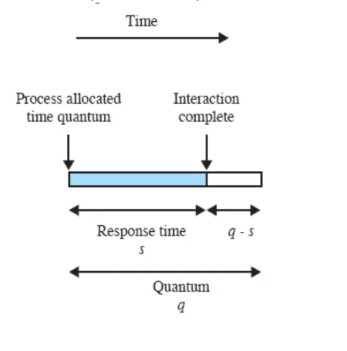
\includegraphics[width=0.75\textwidth]{immagini/Quanto di tempo Giusto}
        \caption{Quanto di tempo piú grande del tempo di interazione}
    \end{figure}
    Se invece uno sceglie il quanto di tempo piú piccolo, il processo che va in esecuzione avrebbe bisogno di piú tempo del quanto,
    prima della risposta gli viene tolto il processore, questo significa che il tempo di risposta é piú lungo.
    \begin{figure}[H]
        \centering
        \includegraphics[width=0.75\textwidth]{immagini/Quanto piú piccolo}
        \caption{Quanto di tempo piú piccolo del tempo di interazione}
    \end{figure}
    Nel momento in cui si sceglie di usare il round robin, si fa una analisi statistica di quantitá di tempo di esecuzione
    necessaria per i processi per assegnare il quanto di tempo, invece se assegno un quanto di tempo troppo grande, allora
    il round robin diventa un FCFS.
    \subsubsection*{CPU bound vs I/O bound}
    C'é un problema con il round robin, per quello che riguarda i processi CPU bound contro i processi I/O bound,
    anche con il round robin anche i processi CPU bound vengono favoriti, perché i processi CPU bound utilizzano
    tutto il quanto di tempo, mentre i processi I/O bound non utilizzano tutto il quanto di tempo in caso di richiesta
    bloccante, dal punto di vista dell'equitá non va bene, é stata proposta una soluzione \textbf{Round Robin Virtuale}
    che funziona come il round robin, ma se un processo fa una richiesta bloccante, allora il processo non va in una coda
    dei ready dopo aver completato la richiesta di I/O come succede normalmente, invece con il round robin virtuale
    esiste una coda ausiliaria, che accoda i processi che sono stati blocked, dopo di che il dispatcher sceglie prima
    la coda ausiliaria e poi la coda dei ready.
    \begin{figure}
        \centering
        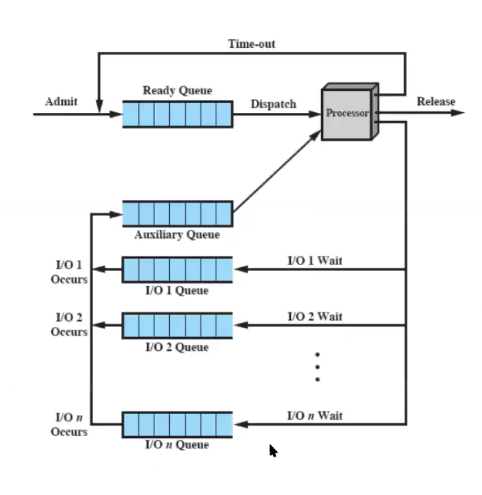
\includegraphics[width=0.75\textwidth]{immagini/RoundRobinVirtuale}
        \caption{Round Robin Virtuale}
    \end{figure}
    Da notare che scegliendo dalla coda ausiliaria, rimando i processi in esecuzione solo per il quanto di tempo che gli rimaneva

    \subsection{Shortest Process Next}
    Il Shortest Process Next é un algoritmo non pre-emptive, per implentarlo é necessario sapere quanto tempo di escuzione il
    processo richiede, la logica per scegliere il prossimo processo é quello col tempo di esecuzione piú breve,
    questo fa si che i processi corti scavalchino i processi piú lunghi.
    \begin{figure}[H]
        \centering
        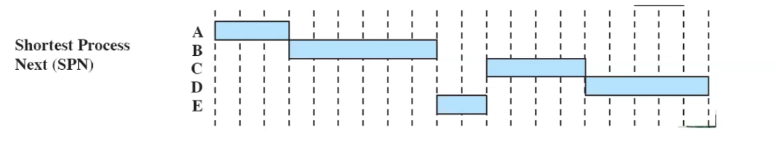
\includegraphics[width=0.75\textwidth]{immagini/SPN}
        \caption{Shortest Process Next}
    \end{figure}
    Il problema é quello di dover dare una stima del tempo di esecuzione dei processi,
    ma anche assumendo di avere una buona stima, dal punto di vista dei criteri utente, la predictability di processi
    lunghi é ridotta, questo addirittura potrebbe creare starvation, perché i processi corti vengono sempre eseguiti
    mentre i processi lunghi potrebbero rimanere in attesa per sempre, se il tempo stimato é sbagliato il sistema operativo
    potrebbe abortire il processo.
    \subsubsection*{Stimare il tempo di esecuzione}
    Per stimare il tempo di esecuzione, ci sono alcuni processi che vengono eseguiti piú volte,
    quindi per questo tipo di processi si puó guardare il passato per prevedere il futuro, ad esempio facendo una
    media dei tempi di esecuzione passati,
    \begin{equation}
    S_n_+_1 = \frac{1}{n} \sum_{i=1}^{n} T_i\label{eq:Media dei tempi di esecuzione}
    \end{equation}
    per fare questo significa che il dispatcher deve tenere traccia del tempo di esecuzione di ogni processo, questo
    potrebbe richiedere molta memoria, l'altro modo é quello di ricordarmi solo l'ultimo tempo di esecuzione e l'ultima
    stime con :
    \begin{equation}
        S_n_+_1 = \frac{1}{n}T_n + \frac{n-1}{n}S_n\label{eq:Mi ricordo solo l'ultimo tempo di esecuzione e l'ultima stima}
    \end{equation}
    questa si puo' generalizzare con un parametro $\alpha$, dove $\alpha$ é un valore tra 0 e 1 otteniamo:
    \begin{equation}
        S_n_+_1 = \alpha T_n + (1-\alpha)S_n\label{eq:formula con $\alpha$}
    \end{equation}
    formula media esponenziale:
    \begin{equation}
        S_n_+_1 = \alpha T_n + ... + (1-\alpha)^iT_n_-_i +...+ (1-\alpha)^nS_1\label{eq: Exponential Averaging }
    \end{equation}
    \begin{figure}
        \centering
        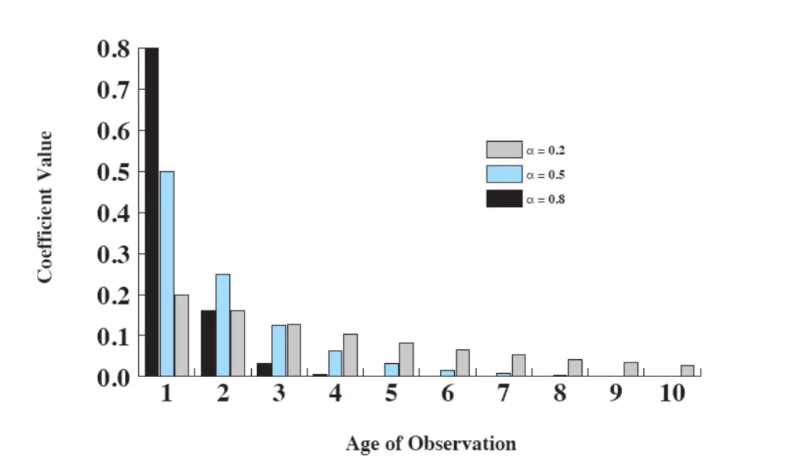
\includegraphics[width=0.75\textwidth]{immagini/AnalisiDiAlphaSpn}
        \caption{Analisi di Alpha}
    \end{figure}
    Piú $\alpha$ é vicino a 1, piú sparisce velocemente il passato, questo serve a capire che con un buon $\alpha$ si 
    possono fare delle ottime previsioni.
    \subsubsection*{Esempio}
    \begin{figure}[H]
        \centering
        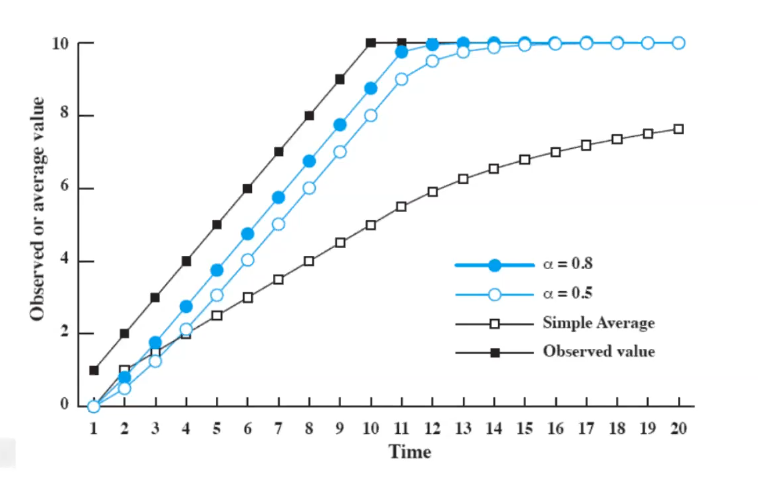
\includegraphics[width=0.75\textwidth]{immagini/EsempioExponentialAveraging}
        \caption{Esempio 1}
    \end{figure}
    Abbiamo fissato un processo e diciamo che la sua prima istanza cresce e poi si stabilizza, se io facessi
    semplicemente la media, quello che la media predirebbe sarebbe un valore lontano dall'obbiettivo, invece
    se uso degli $\alpha$ fissi, siamo molto piú vicini alla curva reale.
    \begin{figure}[H]
        \centering
        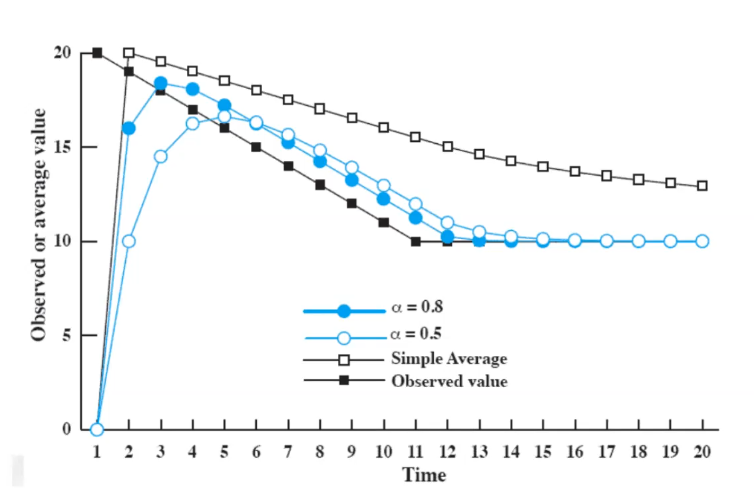
\includegraphics[width=0.75\textwidth]{immagini/EsempioExponentialAveraging2}
        \caption{Esempio 2}
    \end{figure}
    Praticamente dopo un certo tempo, i valori vecchi vengono dimenticati, specialmente per $\alpha$ grandi
    \subsection{Shortest Remaining Time}
    Lo Shortest Remaining Time é una versione pre-emptive dello Shortest Process Next, é preemptive sulla base che arrivi
    un nuovo processo, quindi io stimo il tempo rimanente per l'esecuzione, se il tempo rimanente di un processo in coda é minore
    del tempo di esecuzione del processo in esecuzione, allora il processo in esecuzione viene pre-empted.
    \begin{figure}[H]
        \centering
        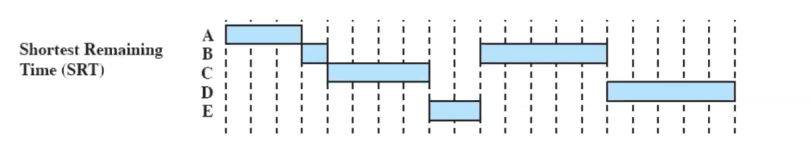
\includegraphics[width=0.75\textwidth]{immagini/SRT}
        \caption{Shortest Remaining Time}
    \end{figure}
    I processi lunghi comunque possono soffrire di starvation, perché i processi corti vengono sempre eseguiti, anche in
    questo caso é necessario sapere il tempo di esecuzione.
    \subsection{Highest Response Ratio Next}
    L' algoritmo Highest Response Ratio Next é un algoritmo non pre-emptive, é una versione migliorata dello Shortest Process Next,
    che risolve il problema dello starvation, é basato sul tempo di attesa, il tempo di esecuzione e il tempo totale richiesto,
    é un compromesso tra quanto tempo sto aspettando e quanto tempo ci metto ad eseguire.

    L'algoritmo massimizza il seguente rapporto:
    \begin{equation}
        \frac{w+s}{s} = \frac{tempo trascorso in attesa + tempo totale richiesto}{tempo totale richiesto}
    \end{equation}
    \begin{figure}[H]
        \centering
        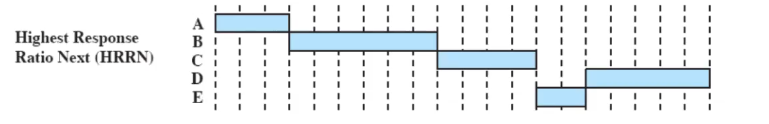
\includegraphics[width=0.75\textwidth]{immagini/HRRN}
        \caption{Highest Response Ratio Next}
    \end{figure}
    \subsectioni*{Diagramma Riassuntivo}
    \begin{figure}[H]
        \centering
        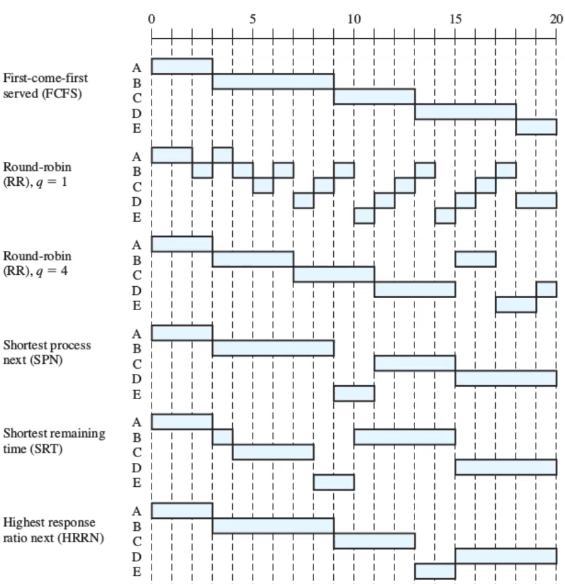
\includegraphics[width=0.75\textwidth]{immagini/RiassuntoScheduling}
        \caption{Diagramma Riassuntivo}
    \end{figure}
    \subsection{Scheduling in Unix}
    Unix combina prioritá e ruond robin, un processo quindi resta in esecuzione per al massimo un secondo, a meno che non termini
    o si blocchi, esistono diverse code a seconda della prioritá; all'interno di ciascuna coda viene eseguito il round robin.
    Le prioritá vengono ricalcolate ogni secondo, piú un processo resta in esecuzione, minore sará la sua prioritá quando
    viene rimesso in coda(feedback). Le prioritá iniziali vengono assegnate in base al tipo di processo :
    \begin{itemize}
        \item swaper (alta)
        \item controllo di un dispositivo di I/O a blocchi
        \item gestione di file
        \item controllo di un dispositivo di I/O a caratteri
        \item processi utente (basso)
    \end{itemize}
    la formula per lo scheduling é
    \begin{equation}[H]
        CPU_j(i)= \frac{CPU_J(i-1)}{2}
    \end{equation}
    che viene poi utilizzata nella formula per il calcolo della prioritá
    \begin{equation}[H]
        P_j(i) = Base_Priority_j + CPU_j(i) + Nice_j
    \end{equation}
    \begin{itemize}
        \item \textbf{J} é un indice che indica i processi \textbf{ready}
        \item \textbf{Base\_Priority\_j} é la prioritá iniziale del processo (da 0 a 4)
        \item \textbf{Nice\_j} Ricordano che il valore della prioritá piú é alto piú la prioritá é bassa, l'idea
        dietro di nice_j é la capacitá di un processo di auto-declassarsi, é usata  nei processi di sistema.
        \item \textbf{CPU\_j(i)} É una misuta di quanto il processo j ha usato il processore nell'intervalli i, con
        exponential averaging dei tempi passati, in particolare con \alpha = \frac{1}{2}
    \end{itemize}
    \subsubsection*{Esempio}
    \begin{figure}
        \centering
        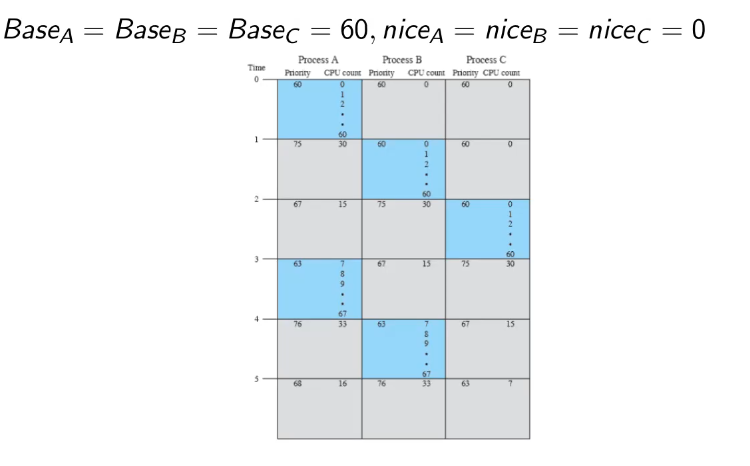
\includegraphics[width=0.75\textwidth]{immagini/EsempioSchedulingUnix}
        \caption{Esempio Scheduling Unix}
    \end{figure}
    Supponiamo che ci siano 3 processi, A, B e C, con il nice = 0 e la base priority = 60, e che il processo A sia in esecuzione
    quindi si comincia da 60 e poi bisogna aggiungere CPU_j che inizialmente é 0, chi non é in esecuzione (B e C) non lo incrementana,
    se il processo A é in esecuzione per un secondo, allora CPU_j = 30 (applicare la formula), finito il tempo di esecuzione,
    si calcola la nuova prioritá (P_j) e si rimette in coda, dopo di che lo scheduler controlla il processo con la prioritá piú alta,
    dopo un secondo quando vengono ricalcolate le prioritá, la prioritá di A diventa 67 perché:
    \begin{equation}
        CPU_j(60) = \frac{60}{2} = 15
    \end{equation}
    \begin{equation}
        P_j = 60 + \frac{CPU_j}{2} + 0 = 75
    \end{equation}
    questa operazione viene fatta per tutti i processi ogni secondo.
    Il Round robin é virtuale, quindi se un processo é bloccato, non viene messo in coda, ma viene messo in una coda ausiliaria,
    e viene eseguito prima di quelli in coda quando torna disponibile.
    \subsection{Architetture Multicore}
    Ci sono diversi modi per avere piú modi per avere piú core:
    \begin{itemize}
        \item \textbf{Cluster} : ogni processore ha la propria RAM
        \item \textbf{Processori specializzati}: un processore per le operazioni di I/O, un processore per le operazioni di calcolo
        \item \textbf{Multi-processore}: Condividono la stessa RAM,un solo sistema operativo controlla tutto
    \end{itemize}
    Noi ci concentreremo sui multi-processori, nel caso di un sistema mono-processore, ho n processi e decido quale di
    essi va in esecuzione, nel caso di un sistema multi-processore, ho n processi e m processori, quindi devo decidere
    se devo fare un Assegnaemnto Statico o Dinamico.
    \subsubsection*{Assegnamento Statico}
    Con l' assegnamento statico, ad ogni processo viene assegnato un processore, per tutta la sua durata andrá in esecuzione su quel
    processore, si puó anche usare uno scheduler per ogni processore, i vantaggi sono che é facile da implementare, ma il problema
    é che un processore potrebbe rimanere idle.
    \subsubsection*{Assegnamento Dinamico}
    Per migliorare lo svantaggio dello statico, un processo, nel corso della sua vita, potrá essere eseguito su diversi processori
    , il sistema operativo potrebbe essere sempre eseguito su un processore fisso, questa cosa é semplice da realizzare mentre solo i processi
    utenti possono essere assegnati a processori diversi, un altra scelta é quella di eseguire il sistema operativo su tutti i processori
    ma questo causa piú overhead.
    \subsection{Scheduling in Linux}
    Linux cerca la velocitá di esecuzione, tramite semplicitá, per questo non esiste long-term e medium-term scheduler (non
    ha senso perché non esistono processi suspended), Un embrione del long-term c'é perché quando creo un processo il sistema
    potrebbe essere giá saturo.
    \subsubsection*{Come Funziona}
    Ci sono le runqueue(Code dei Ready), e le wait queues (code dei blocked), Le wait queues sono condivise tra i processori,
    mentre le runqueue sono separate, ogni processore ha la sua runqueue. Essenzialmente lo scheduling é derivato da quello
    di UNIX, quindi é pre-emptive, a prioritá dinamica, ma con importanti correzzioni :
    \begin{enumerate}
        \item essere veloce, ed operare quasi in O(1)
        \item servire in modo appropriato i processi real-time
    \end{enumerate}
    Linux istruisce l'hardware di mandare un timer interrupt ogni 1ms:
    \begin{itemize}
        \item piú lungo abbiamo problemi per appicazioini real-time
        \item piú corto arrivano troppi interrupt, per cui abbiamo tanto tempo speso in Kernel Mode e quindi meno tempo
        per i processi utenti
    \end{itemize}
    percui il quanto di tempo per ciascun processo é un multiplo di 1ms.\\


    Linux considera tre tipi di processi:
    \begin{itemize}
        \item \textbf{Real-time} : hanno prioritá fisse, e vengono eseguiti prima di tutti gli altri
        \item \textbf{Interattivi} : hanno prioritá dinamiche, e vengono eseguiti dopo i real-time
        \item \textbf{Batch} : hanno prioritá dinamiche, e vengono eseguiti dopo gli interattivi
        \end{itemize}
    \subsubsection*{Interattivi}
    Non appena si agisce sul mouse o sulla tastier, é importante dare lor la CPU in 150ms al massimo
    \subsubsection*{Batch}
    Lo scheduler puó decidere di penalizzare i processi batch, perché non sono interattivi, quindi non c'é bisogno di dare
    un feedback immediato all'utente.
    \subsubsection*{Real-time}
    Gli unici riconosciuti come tali da Linux: Il loro codice sorgente usa la system call \textbf{sched\_setscheduler}
    ,per gli altri usa un'euristica, esempi di sistemi real-time sono riproduttori di audio e video, controllori, ... ma normalmente
    sono usati dai KLT.
    \subsubsection*{Classi di scheduling}
    Linux ha 3 classi di scheduling:
    \begin{itemize}
        \item \textbf{SCHED\_FIFO e SCHED\_RR } : fanno riferimento ai processi real-time
        \item \textbf{SCHED\_OTHER} : fanno riferimento a tutti gli altri processi
    \end{itemize}
    Prima si eseguono quelli che sono in SCHED\_FIFO e SCHED\_RR, poi quelli in SCHED\_OTHER, le prime due classi hanno
    un livello di priorità che va da 1 a 99, mentre la terza classe ha un livello di priorità che va da 100 a 139,
    quindi ci sono 140 runqueues per ogni cpu, si passa dal livello n al ilvello al livello n+1 solo se o non ci sono processi in n,
    o nessun processo in n é in RUNNING.\\

    La preemption puó essere dovuta a:
    \begin{itemize}
        \item si é esaurito il quanto di tempo
        \item un altro processo passa da blocked a RUNNING, questo succede quando c'é un processo interattivo bisogna cercare di eseguirlo il prima possibile
    \end{itemize}
    Molto spesso, il processo che é appena diventato eseguibile sará quello eseguito dal processore, questo é dovuto al fatto
    che il processo é stato bloccato per un I/O, quindi é probabile che sia un processo interattivo.
    \subsubsection*{Regole generali}
    Un processo SCHED\_FIFO viene non solo preempted, ma anche rimesso in coda solo se:
    \begin{itemize}
        \item si blocca per I/O
        \item un processo passa da uno degli stati blocked a RUNNING, ed ha prioritá maggiore
        \end{itemize}
    Un processo SCHED\_RR viene preempted per i motivi dello SCHED\_FIFO, ma anche se il quanto di tempo é scaduto (RR = RoundRobin).


    I processi real-time hanno una prioritá fissa, e non possono essere preempted da processi con prioritá dinamica, invece i
    processi SCHED\_OTHER si con un meccanismo simile a quello di UNIX, inoltre per sistemi multiprocessore esiste una
    routine per distribuire il carico.
    
    \section{Gestione della Memoria}
    La memoria é oggi a basso costo, e con trend in diminuzione, questo fa si che le applicazioni usino sempre piú memoria,
    se ogni processo dovesse gestire la propia memoria, ogni processo userebbe semplicemente tutta la memoria disponibile,
    questo porterebbe all'assenza della multiprogrammazzione che é un aspetto essenziale per il corretto funzionamento del
    sistema operativo, si potrebbe imporre dei limiti di memoria a ciascun processo, diventa peró difficile per un programmatore
    scrivere un processo che rispetti tali limiti, quindi ogni sistema operativo deve avere un sistema di gestione della memoria
    cercando di dare l'illusione ai processi di avere tutta la memoria, la soluzione é quella di usare il disco come buffer
    per memoria, questa gestione di I/O é ovviamente piú lenta del processore, per cui il SO deve pianificare lo swap
    \subsection{Requisiti}
    \begin{itemize}
        \item Rilocazione : importante che ci sia aiuto hardware, aiuto, non gestione diretta per cui sistema operativo e hardware collaborano
        \item Protezione : importante che ci sia un aiuto hardware
        \item Condivisione
        \item Organizzazione logica
        \item Organizzazione fisica
    \end{itemize}
    \subsubsection{Rilocazione}
    Il programmatore non sa e non deve sapere in quale zona della memoria il programma verrá caricato :
    \begin{itemize}
        \item potrebbe essere swappato su disco, e al ritorno in memoria principale potrebbe essere caricato in un'altra zona
        \item potrebbe anche non essere contiguo, oppure con altre pagine in RAM e altre in disco
        \item in questo contesto, si intende chi usa l'assembler o il compilatore
    \end{itemize}
    I riferimente alla memoria devono essere tradotti nell'indirizzo fisico : preprocessing, run-time,se run-time occrre supporto hardware
    \begin{figure}[H]
        \centering
        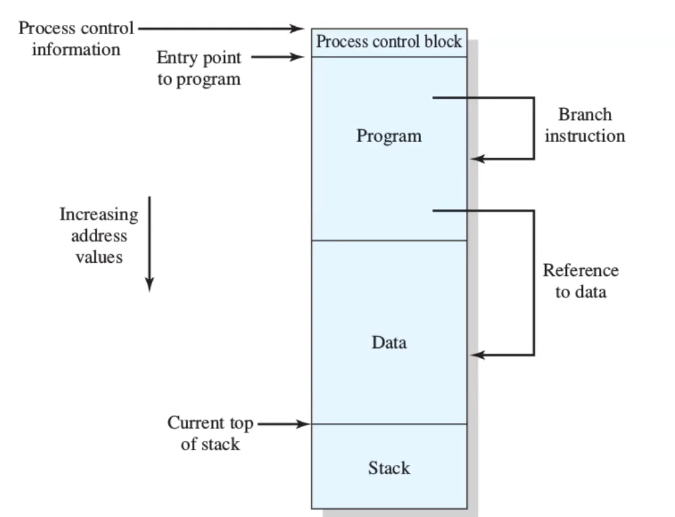
\includegraphics[width=0.75\textwidth]{immagini/RilocazioneIndirizziNeiProgrammi}
        \caption{Rilocazione}
    \end{figure}
    un processo ha una zona con il programma in liguaggio macchina, e una zona con i dati, e una zona con lo stack, la sua parte iniziale
    é il PCB, gli indirizzi che possiamo avere sono indirizzi di salto oppure referenze a variabili, tutti questi inidirizzi
    devono essere ricalcolati.
    \subsubsection*{Indirizzi nei programmi}
    \begin{figure}[H]
        \centering
        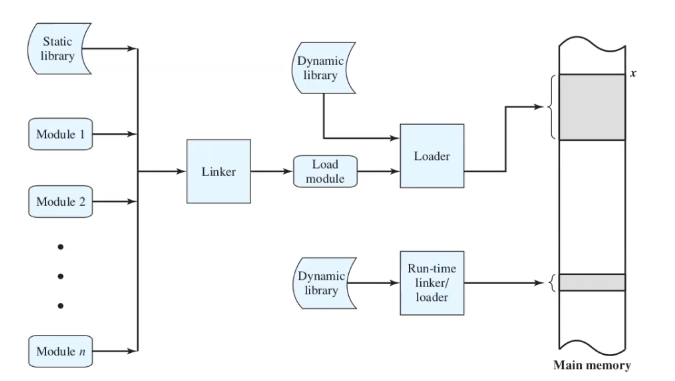
\includegraphics[width=0.75\textwidth]{immagini/Indirizzi nei programmi}
        \caption{Indirizzi nei programmi}
    \end{figure}
    Per capire come avviene la rilocazione dobbiamo prima precisare... Un programma eseguibile viene prima scritto
    in moduli, uno di questi moduli ha il main, quindi ci sono tanti moduli scritti dal programmatore oppure librerie
    , ognuno di questi moduli viene compilato separatamente, ed per ogni modulo viene creato un file oggetto, tutto
    questo viene collegato attraverso il linker in modo da creare un file eseguibiler (nell'esempio Load module),
    poi c'é il loader che carica il file eseguibile in memoria, nel fare questo ci potrebbe essere bisogno di alcune librerie dinamiche
    \begin{figure}[H]
        \centering
        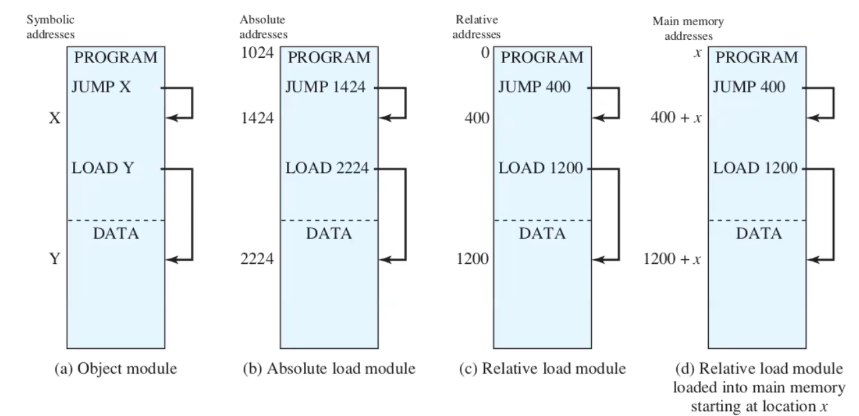
\includegraphics[width=0.75\textwidth]{immagini/IndirizziInMemoria}
        \caption{Effettivo in memoria}
    \end{figure}
    Il risultato é mostrato nell'immagine, ogni singolo modulo ha la sua parte di programma e la sua parte di dati,
    sostanzialmente il programma contiene soltanto indirizzi simbolici, quando peró viene trasformato in un file eseguibile
    abbiamo 2 possibilitá:
    \begin{itemize}
        \item Indirizzo Assoluto : Lui sa che deve cominciare a 1024, e se deve saltare a 1424, il loader deve caricare il programma all'indirizzo 1024 altrimenti non funziona.
        \item Indirizzo Relativo : Con gli inderizzi relativi, si puó suppore di partire da 0, e nel caso di un salto scrivo solo l'indirizzo rispetto all'inizio del programma.
    \end{itemize}
    \subsubsection*{Tipi di Indirizzi}
    \begin{itemize}
        \item \textbf{Indirizzi Logici} : vengono usati dal programmatore, sono indirizzi simbolici, non sono reali, sono rilocati
        \item \textbf{Indirizzi Fisici} : sono gli indirizzi reali, sono quelli che vengono usati dal processore
        \item \textbf{Indirizzi Relativi} : il riferimento é espresso come un un spiazzamento rispetto ad un punto di riferimento.
    \end{itemize}
    \begin{figure}[H]
        \centering
        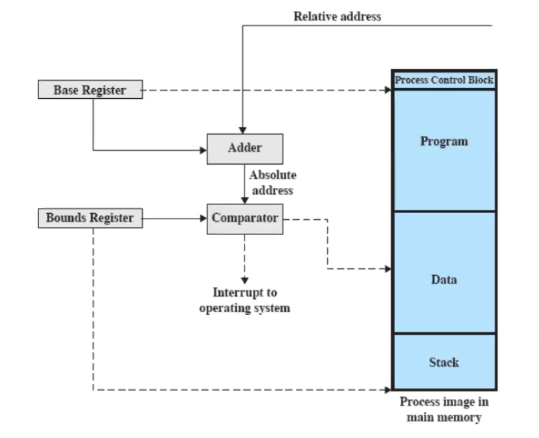
\includegraphics[width=0.75\textwidth]{immagini/RilocazioneConHardware}
        \caption{Tipi di Indirizzi}
    \end{figure}
    Nel caso di indirizzi relativi, l' hardware della macchina sa che se per esempio abbiamo un salto a 100, allora
    l'hardware sa che deve sommare 100 all'indirizzo base (Es. 6000), quindi l'indirizzo fisico sará 6100, inoltre c'é una
    fase di controllo per rimanere nei limiti di memoria, e fondamentale che ogni volta che il sistema operativo carica il
    processo il sistema operativo deve preoccuparsi di mettere l'indirizzo corretto nel base register.\\

    I registri usati sono:
    \begin{itemize}
        \item Base Register : contiene l'indirizzo base del processo.
        \item Limit Register : contiene l'indirizzo di fine del processo.
    \end{itemize}
    I valori per questi registri vengono settati nel momento in cui il processo viene posizionato in memoria, mantenuti nel PCB del processo,
    fa parte del passo 6 del process switch e non vanno semplicemente modificati occore propio modificarli.
    \subsubsection{Protezione}
    I processi non devono poter accedere alla locazione di memoria di memoria di un'altro processo, a meno che
    non sia stato esplicitamente condiviso, A causa della rilocazione non puó essere fatto a tempo di compilazione,
    pertanto serve un supporto hardware.
    \subsubsection{Condivisione}
    La condivisione deve essere possibile, permettere a piú processi di accedere alla stessa locazione di memoria, solo se é effettivamente
    utile allo scopo perseguito, c'é anche casi in cui é il sistema operativo in maniera trasparente, il caso tipico é quando
    si seseguono piú processi eseguendo lo stesso codice sorgente, quindi lo metto in RAM una volta sola.
    \subsubsection{Organizzazione Logica}
    A livello hardware, la memoria é organizzata in modo lineare, A livello software , i programmi sono scritti in moduli,
    per cui il SO deve offrire tali caratteristiche, facendo da ponte tra la prima visuale (moduli) e la seconda (lineare).
    \subsubsection{Organizzazione Fisica}
    L' organizzazione fisica é quella che si occupa del flusso di dati tra RAM e la memoria secondari, questa non é una
    cosa lasciata al programmatore, se per esempio io scrivo un programma che necessitá di 1GB di ram ma il sistema
    operativo me ne assegna 500MB, una volta il programmatore doveva usare l'overlay per suddividere il programma in
    pezzi e gestire lo swap tra ram e disco in maniera manuale, oggi il sistema operativo si occupa di tutto ció.
    \subsection{Partizionamento}
    Uno dei primi metodi per gestire la memoria é il partizionamento, la memoria viene divisa in partizioni, esso
    puó essere di diversi tipi:
    \begin{itemize}
        \item \textbf{Partizionamento Fisso} : la memoria é divisa in partizioni di dimensione fissa.
        \item \textbf{Partizionamento Dinamico} : la memoria é divisa in partizioni di dimensione variabile.
        \item \textbf{Paginazione Semplice} : la memoria é divisa in pagine di dimensione fissa.
        \item \textbf{Segmentazione Semplice} :
        \item \textbf{Paginazione con memoria virtuale} :
        \item \textbf{Segmentazione con memoria virtuale} :
    \end{itemize}
    \subsubsection{Partizionamento Fisso Uniforme}
    Quando accendo il sistema operativo, tra le cose che vengono fatte il SO divide la memoria in partizioni di dimensione
    fissa, 1 é riservata al kernel, le altre sono per i processi, l'idea é quella di mettere al loro interno i processi
    che peró non possono superare la partizione assegnata all'inizio, chiaramente il SO puó decidere se sospendere
    e quindi spostare il processo sul disco, in questo caso era il programmatore a dover essere sicuro di non sforare
    la partizione assegnata.
    \subsubsection*{Problemi}
    un programma potrebbe non entrare in una partizione, questo porta anche ad un uso inefficiente della memoria, perché
    porta al fenomeno della frammentazione interna.
    \subsubsection{Partizionamento Fisso Variabile}
    Nel partizionamento variabile comunque le partizioni vengono assegnate una sola volta, ma la dimensione delle partizioni
    é variabile, questo permette di mettere i processi piú leggeri in partizioni piú piccole.
    \subsubsection*{ALgoritmo di Posizionamento}
    Da momento in cui ho partizioni di dimensioni variabili, mi devo preoccupare di dove mettere i processi, una scelta
    é quella di avere una coda per partizione , oppure ho una unica coda e mano a mano assegno alla partizione che spreca
    meno spazio, se uso la coda unica posso fare delle ottimizzazioni nel senso che piuttosto che non far eseguire un
    processo lo carico in memoria, anche se spreco un po' di memoria.
    \begin{figure}[H]
        \centering
        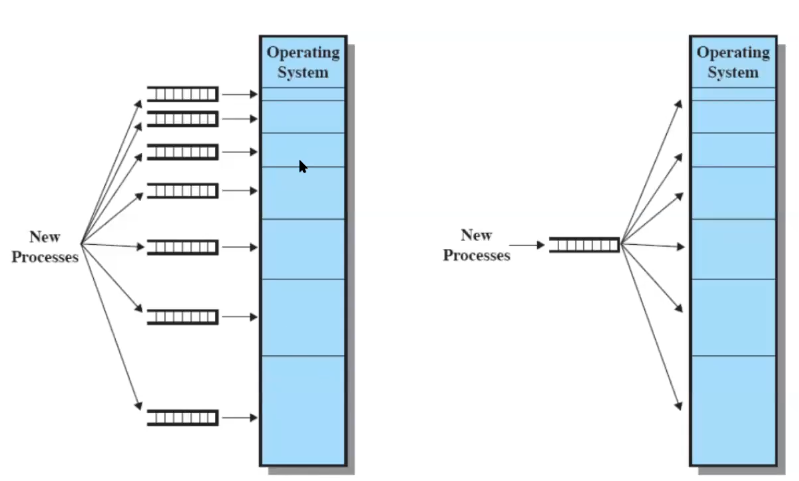
\includegraphics[width=0.75\textwidth]{immagini/partizionamento}
        \caption{Partizionamento Variabile}
    \end{figure}
    \subsubsection*{Problemi Irrisolti}
    C'é un numero massimo di processi in memoria principale dettato dal fatto che il numero di processi non puó superare
    il numero di partizione, inoltre la gestione della memoria risulta comunque inefficiente se ho tanti processi piccoli.
    \subsubsection{Partizionamento Dinamico}
    Le partizioni variano sia in misura che in quantitá, la dimensione delle partizione varia in base alla dimensione 
    del processo.
    \subsubsection*{Esempio}
    \begin{figure}[H]
        \centering
        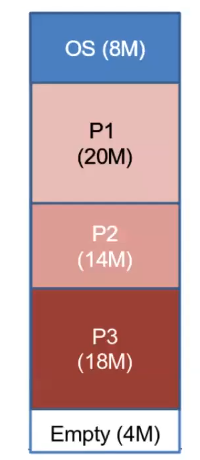
\includegraphics[width=0.25\textwidth]{immagini/EsempioPartizionamentoDinamico}
        \caption{Partizionamento Dinamico}
    \end{figure}
    Supponiamo che arrivino in sequenza tre processi, p1=20MB, p2=14MB, p3=18MB, stiamo
    assumendo che chiaramente stiamo usando indirizzi relativi, in una memoria da 56M
    resta un blocco da 4MB, se arriva un processo da 5MB, il sistema operativo deve fare una
    scelta, supponiamo che il processo da 5MB sia il processo p4 e sia piú importante di p2
    \begin{figure}[H]
        \centering
        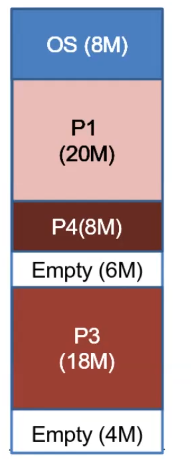
\includegraphics[width=0.25\textwidth]{immagini/EsempioPartizionamentoDinamico2}
        \caption{Partizionamento Dinamico}
    \end{figure}
    quello che succede é che si lascia uno spazio vuoto di 6MB, p2 chiaramente viene copiato
    sul disco in attesa che venga richiamato, ora peró vogliamo far eseguire p2 che é piú importante
    di p1 copiamo p1 sul disco e carichiamo p2 in memoria, ora abbiamo un ulteriore spazio vuoto di 6MB
    \begin{figure}[H]
        \centering
        \includegraphics[width=0.25\textwidth]{immagini/EsempioPartizionamentoDinamico3}
        \caption{Partizionamento Dinamico}
    \end{figure}
    si nota che ci sono 16MB di spazio vuoto, se arriva un processo da 10MB, non
    lo posso eseguire perché la memoria non é contigua.
    \subsubsection*{Problemi}
    La frammentazione esterna é un problema, che peró si puó risolvere con la compatazzione. \\

    se ho piú blocchi liberi, ed arriva un processo che potrebbe entrare in uno di questi blocchi, il sistema operativo
    utilizza un algoritmo per scegliere il blocco in cui mettere il processo, l'algoritmo puó essere:
    \begin{itemize}
        \item First Fit : metto il processo nel primo blocco che trovo
        \item Best Fit : metto il processo nel blocco piú piccolo che trovo
        \item Worst Fit : metto il processo nel blocco piú grande che trovo
    \end{itemize}
    \subsubsection*{Best Fit}
    l'algoritmo Best Fit ad una prima valutazione potrebbe sembrare il migliore, ma in realtá é il peggiore, perché
    lascia tanti piccoli blocchi liberi, che non possono essere usati.
    \subsubsection*{First Fit}
    \begin{enumerate}
        \item scorre la memoria dall'inizio; il primo blocco con abbastanza spazio viene usato
        \item é molto veloce
        \item tende a riempire solo la prima parte della memoria
        \item A conti fatti era il migliore
    \end{enumerate}
    \subsubsection{Next Fit}
    Next Fit é una variante di First Fit, la differenza é che Next Fit ricorda dove ha finito l'ultima volta, e riparte
    dall'ultima appena asseggnate per evitare che solo la prima parte della memoria venga usata, assegna piú spesso
    l'ultimo blocco di memoria.
    \begin{figure}[H]
        \centering
        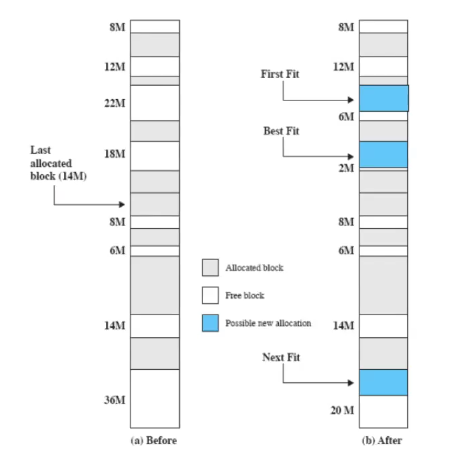
\includegraphics[width=0.75\textwidth]{immagini/AlgoritmiPartizionamento}
        \caption{Confronto tra algoritmi}
    \end{figure}
    \subsubsection{Buddy System}
    Il Buddy system é ancora partizionamento, in questo caso é un compromesso tra partizionamento fisso e dinamico,
    é ancora usato nei sistemi operativi moderni, esempio : supponiamo che 2^U la dimensione di memoria di memoria
    a disposizione per l'utente e che \textbf{s} sia la dimensione di un processo, quello che fa il buddy system é
    dividere per 2 fino a che non si arriva alla dimensione tale che:
    \begin{equation}
        2^(X-1) <= s <2^x
    \end{equation}
    Una delle 2 porzioni é usata per il processo, L' invece serve per dare un lower bound, ovvero non si potranno creare
    partizioni troppo piccole, quando il processo finisce, se il buddy é libero, si uniscono.\\

    Esempio: supponiamo di avere un blocco da 1 MB, e che arrivi un processo da 100KB, quindi andiamo a dividere
    il blocco per 2, ed osserviamo di avere 2 blocchi da 512KB, il blocco é ancora troppo grande, ne prendiamo uno
    e lo dividiamo per 2, ottenendo 2 blocchi da 256KB, il blocco é ancora troppo grande, ne prendiamo uno e lo dividiamo
    per 2, ottenendo 2 blocchi da 128KB, il blocco adesso é della dimensione corretta perché se divido ancora per 2 i 2 blocchi
    risultanti saranno troppo piccoli per ospitare il processo,ci sará quindi una frammentazione interna di 28KB, supponiamo
    ora  che arrivi un processo da 240KB, vediamo che dalla divisione di prima é avanzato un blocco da 256KB e quindi
    quella partizione viene usata, ora supponiamo che arrivi un processo da 64KB, dividiamo il blocco da 128KB e selezioniamo
    uno dei due blocchi da 64KB, per ricreare le partizioni quando un processo termina, l'idea é quella di riaccoppiare i blocchi
    con i propri buddy, quindi se un blocco da 64KB termina, si unisce con il blocco da 64KB, e tutti e due devono derivare
    dallo stesso blocco da 128KB e cosi via fino a riformare il blocco da 1MB.
    \begin{figure}[H]
        \centering
        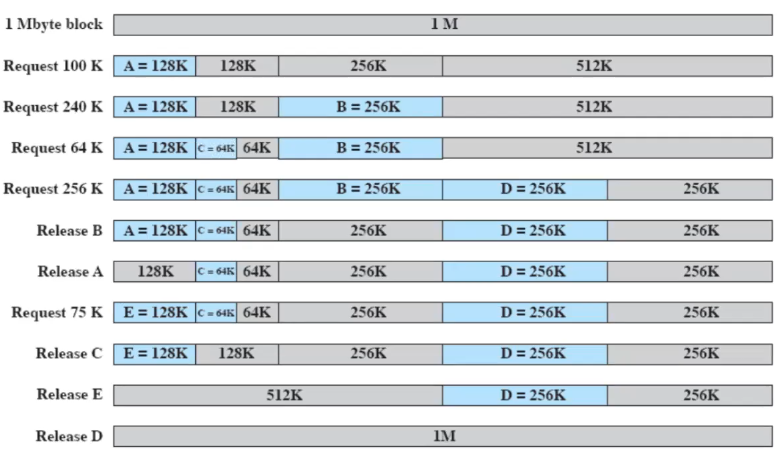
\includegraphics[width=0.75\textwidth]{immagini/BuddySystem1}
        \caption{Buddy System}
    \end{figure}
    Da notare che il buddy system si presta bene per essere rappresentato come un albero binario, quindi
    per migliorare la ricerca si implementava la ricerca tramite bynary search tree, in questo modo si evita di scorrere tutta
    la memoria.
    \begin{figure}[H]
        \centering
        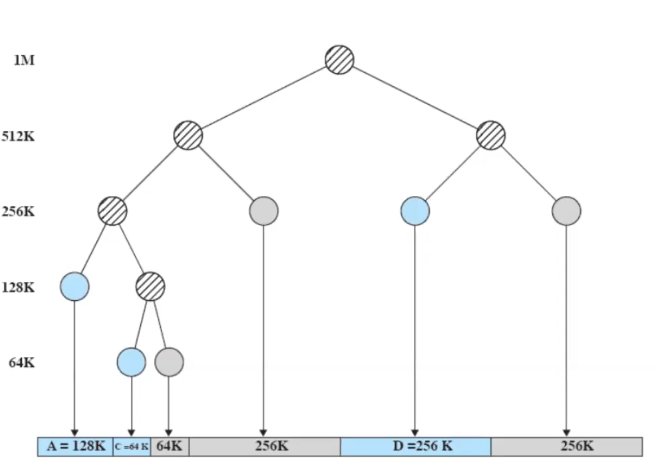
\includegraphics[width=0.75\textwidth]{immagini/BuddySystemAlbero}
        \caption{Buddy System}
    \end{figure}
    \subsection{Paginazione}
    \subsubsection*{Paginazione Semplice}
    Sia la memoria che i processi vengono divisi in pezzi di dimensione fissa e piccola (1KB), questo si fa sia
    con la RAM che con i processi, se un processo é grande 1MB viene diviso in 1024 pezzi (1KB), questi pezzi
    sono chiamati pagine per i processi, mentre i pezzetti di memoria sono chiamati frame, La cosa essenziale
    che ogni pagina per essere utilizzata deve essere collacata in un frame, la cosa interessante che pagine
    contigue non devono essere collocate in frame contigui, questo permette di evitare la frammentazione interna,
    tutto il processo é trasparente al programmatore, a questo punto serve che i sistemi operativi mantengano
    una tabella che mappi le pagine ai frame, questa tabella é chiamata Page Table, questo punto peró bisogna
    correggere gli indirizzi, per cui c'é bisogno di un supporto hardware.
    \subsubsection*{Esempio}
    Supponiamo che arrivi un processo \textbf{A} che richiede 4 frame, poi \textbf{B} da 3 frame, e poi \textbf{C} da
    4 frame, poi il processo \textbf{B } termina, quello che succederebbe se fossimo in partizionamento dinamico ed
    arrivasse un processo da 5 dovrei eseguire la compattazione, in questo caso invece posso usare i 3 frame che
    erano stati assegnati a \textbf{B} per il processo \textbf{D}, ed i restanti 2 frame li posso accodare a C.
    \begin{figure}[H]
        \centering
        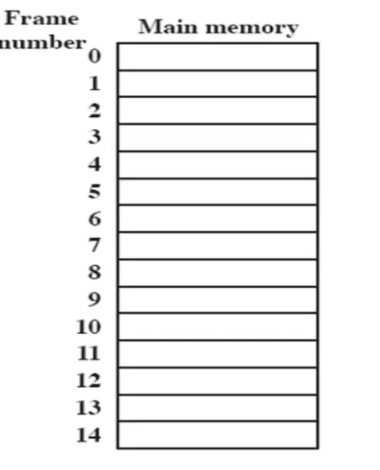
\includegraphics[width=0.5\textwidth]{immagini/PaginazioneEsempio1}
    \end{figure}
    \begin{figure}[H]
        \centering
        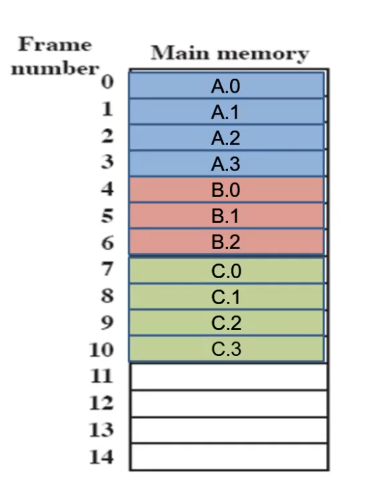
\includegraphics[width=0.5\textwidth]{immagini/PaginazioneEsempio1and2}
    \end{figure}
    \begin{figure}[H]
        \centering
        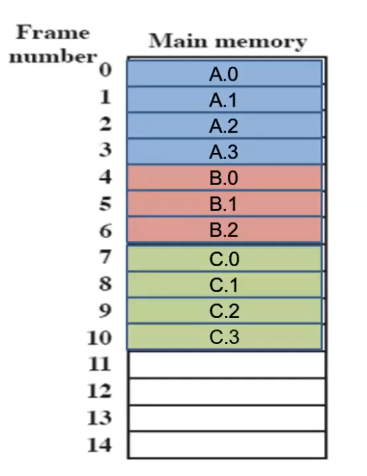
\includegraphics[width=0.5\textwidth]{immagini/PaginazioneEsempio2}
    \end{figure}
    \begin{figure}[H]
        \centering
        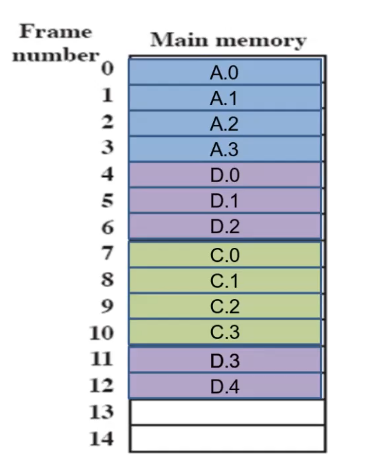
\includegraphics[width=0.5\textwidth]{immagini/PaginazioneEsempio3}
    \end{figure}
    Le tabelle risultanati sono:
    \begin{figure}[H]
        \centering
        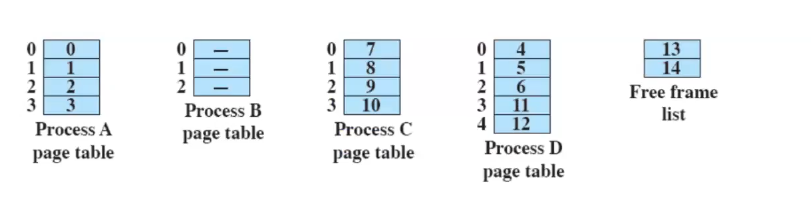
\includegraphics[width=0.75\textwidth]{immagini/PagineRisultanti}
        \caption{Tabelle delle pagine risultanti}
    \end{figure}
    \subsection{Segmentazione}
    \subsubsection*{segmentazione Semplice}
    La differenza tra segmentazione e paginazione é che la segmentazione divide i processi in segmenti di dimensione
    variabile, mentre la paginazione divide i processi in pagine di dimensione fissa, la differenza é che
    il programmatore a dover dividere il processo in segmenti(Sorgenti,Dati,\ldotsecc), dichiarando quali segmenti ci sono e qualé la loro dimensione
    a caricarli in memoria ed a risolvere gli indirizzi é il sistema operativo, sempre con l'aiuto dell'hardware.
    \subsection{Indirizzi Logici}
    Dobbiamo quindi considerare una rivisitazione degli indirizzi logici,
    con gli indirizzi relativi ad esempio, il programmatore sa che il suo programma inizia a 0, e che se deve saltare
    a 100, deve scrivere 100 poi é il sistema operativo che aggiunge l'offset necessari per andare
    all'istruzione corretta,Supponiamo quindi di avere un processo diviso in 3 pagine (notare che é presente
    la frammentazione interna), la prima cosa da fare quindi con un indirizzo é capire in quale pagina si trova dopo
    di che ho un offset rispetto all'inizio della pagina, devo andare ad usare la tabella delle pagine per capire dove
    si trova l'inizio del frame e sommare l'offset, il risultato é l'indirizzo fisico, in maniera analoga
    funziona anche per la segmentazione, da tenere presente che i segmenti hanno dimensione variabile.
    \begin{figure}[H]
        \centering
        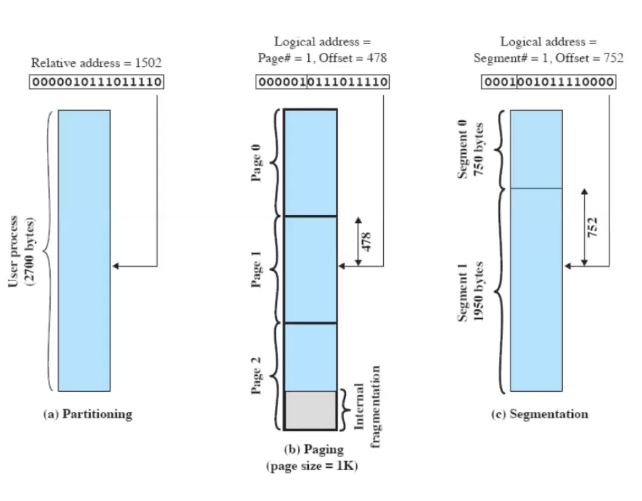
\includegraphics[width=0.75\textwidth]{immagini/IndirizziLogici1}
        \caption{Indirizzi Logici}
    \end{figure}
    \subsubsection*{Paginazione Esempio}
    Supponiamo di essere in una istruzione hardware e questa istruzione harware ha un indirizzo di 16 bit logico,
    quello che devo fare é ricavare l'indirizzo fisico,le dimensioni delle pagine sono sempre un potenza di 2
    allora lascio i primi 10 bit che sono usati per l'offset, mentre i 6 bit piú significativi sono usati per
    capire in quale pagina si trova l'indirizzo questo é vero perché abbiamo preso pagine di dimensione \begin{math}2^1^0\end{math}
    quindi per generalizzare se la dimensione della pagina é \begin{math}2^x\end{math} allora gli x bit meno significativi sono usati
    per l'offset, mentre i bit piú significativi sono usati per capire in quale pagina si trova l'indirizzo, quind una
    volta trovata la pagina, vado a sostituire il contenuto della tabella all'interno dei dei bit che prima erano
    riservati alla tabella, in sostanza i bit piú significativi all'inizio sono usati per contenere l'indirizzo per la
    tabella delle pagine che contiente i bit che servono per trovare l'indirizzo fisico.
    \begin{figure}[H]
        \centering
        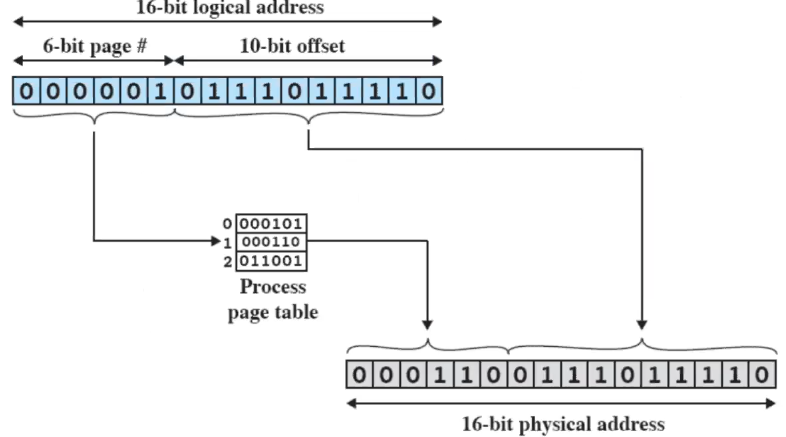
\includegraphics[width=0.65\textwidth]{immagini/funzionamentopaginazione1}
        \caption{}
        \label{fig:funzionamentopaginazione1}
    \end{figure}
    \subsubsection*{Segmentazione Esempio}
    Se voglio tradurre da indirizzo logico a indirizzo fisico, anche in questo caso la lunghezza massima dei segmenti é
    decisa dal sistema operativo, in questo caso siccome ogni segmento ha una dimensione varaibile devo andare a recuperare
    la posizione del segmento nella tabella dei segmenti, e sommare  i bit di offset, inoltre nella tabella é contenuta
    anche la lunghezza del segmento.
    \begin{figure}[H]
    \centering
    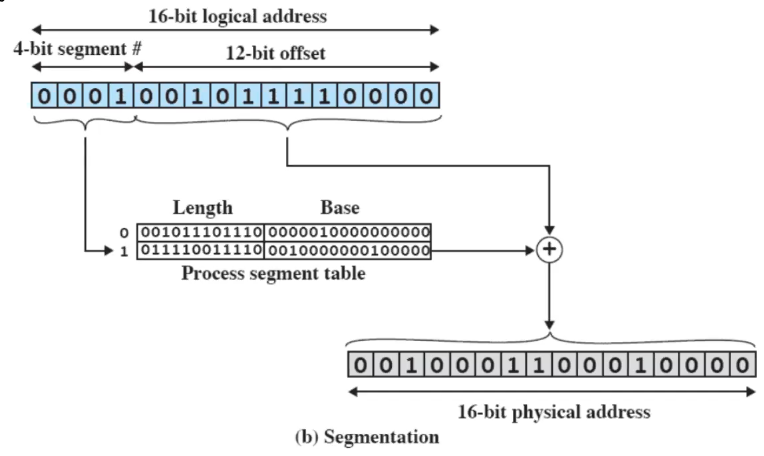
\includegraphics[width=0.65\textwidth]{immagini/indirizzologicosegmentazione}
    \caption{}
    \label{fig:indirizzologicosegmentazione}
    \end{figure}
    \subsection{Memoria Virtuale}
    I riferimenti alla memoria quindi sono indirizzi logici che devono essere tradotti in indirizzi fisici, con
    la paginazione e la segmentazione un processo puó essere diviso in piú parti é puó trovarsi in zone differenti
    della memoria, l'idea é che effettivamente non c'é la necessitá che tutto il processo sia in memoria principale,
    perché quello che serve effettivamente é che la parte del processo che é in esecuzione sia in memoria principale,
    tutto il resto puó essere sul disco,quindi il sistema operativo mette in memoria solo la parte del processo
    che é in esecuzione questo insieme di dati in memoria principale si chiama \textbf{resident set}, se la
    pagina peró non si trova in memoria principale, si verifica un \textbf{page fault}, il sistema operativo
    quindi chiama un interrupt che si occupa di andare a prendere la pagina mancante e metterla in memoria principale,
    fino a che la pagina non é in memoria principale il processo é blocked, quando effettivamente la pagina é effettivamente
    in memoria il processo viene sbloccato e puó continuare l'esecuzione, \textbf{quando il processo verrá eseguito bisognerá
    ri-eseguire l'istruzione che ha causato il page fault}.
    \subsubsection*{conseguenze}
    \begin{itemize}
        \item Ci possono essere molti processi in memoria principale perché basta una pagina in memoria principale
        \item Diventa molto probabile che ci sia un processo ready diminuendo l'idle del processore
        \item Posso eseguire un programma piú grande della memoria principale
    \end{itemize}
    \subsubsection*{Terminologia}
    La Memoria virtuale é uno schema di allocazione di memoria, in cui la memoria secondaria puó essere usata come se
    fosse memoria principale.
    \begin{itemize}
        \item Gli indirizzi usati nei programmi e quelli usati dal sistema sono diversi
        \item C'é una fase di traduzione automatica dai primi indirizzi (logici) ai secondi (fisici)
        \item La dimensione della memoria virtuale é limitata dallo schema di indirizzamento, oltre che
        dalla dimensione della memoria secondaria
        \item la dimensione della memoria principale, non influisce sulla dimensione della memoria virtuale
        \item \textbf{Indirizzo Virtuale} : indirizzo logico
        \item \textbf{Spazio degli indirizzi virtuali} : la quantitá di memoria virtuale assegnata ad un processo
        \item \textbf{Spazio degli indirizzi}: la quantitá di memoria assegnata ad un processo
        \item \textbf{Indirizzo Reale} : indirizzo fisico
    \end{itemize}

    \begin{figure}[H]
        \centering
        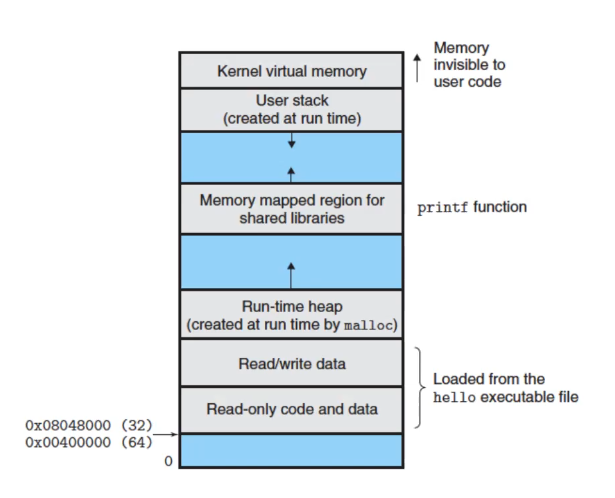
\includegraphics[width=0.65\textwidth]{immagini/comeunprocessovedelamemoria}
        \caption{come un processo vede la memoria}
        \label{fig:comeunprocessovedelamemoria}
    \end{figure}
    \subsubsection{Trashing}
    Il trashing é quando il sistema operativo perde piú tempo a fare swap tra memoria principale e secondaria per
    caricare le pagine che a fare effettivamente il lavoro, per evitarlo il sistema operativo cerca di indovinare quali
    pezzi di processo saranno usati con minore o maggiore probabilitá, nel futuro prossimo,questo tentativo di divinazione
    avviene sulla base della storia recente, sfruttando il principio di localitá (i riferimenti tendono ad essere vicini),
    questo vale sia per i dati che per le istruzioni.
    \subsubsection{Supporto Hardware}
    Paginazione e segmentazione devono essere supportate dall'hardware, in particolare la traduzione degli indirizzi,
    mentre il sistema operativo si occupa di muovere le pagine/segmenti tra memoria principale e secondaria
    \subsubsection*{Paginazione}
    Ogni processo ha una sua tabella delle pagine, il control block di un processo punta a tale tabella, ed ogni entry
    di questa tabella contiene:
    \begin{itemize}
        \item Il numbero di frame in memoria principale
        \item NON c'é il numero di pagina, é direttamente usato per indicizzare la tabella
        \item un bit per indicare se é in memoria principale o meno (Bit di presenza)
        \item un bit per indicare se é stato modificato in seguito all'ultima volta che é stata caricata in memoria (Bit di modifica)
    \end{itemize}
    \begin{figure}
        \centering
        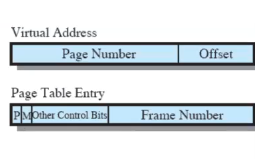
\includegraphics[width=0.65\textwidth]{immagini/pagetableentry}
        \caption{Page Table Entry}
        \label{fig:pagetableentry}
    \end{figure}
    Per quanto riguarda invece l'hardware per la traduzione degli indirizzi, la somma non é una semplice somma: il numero
    di pagina va moltiplicato per il numero di bytes di ogni singola entry della tabella delle pagine, dopo di che si puó
    fare la somma.
    \begin{figure}[H]
        \centering
        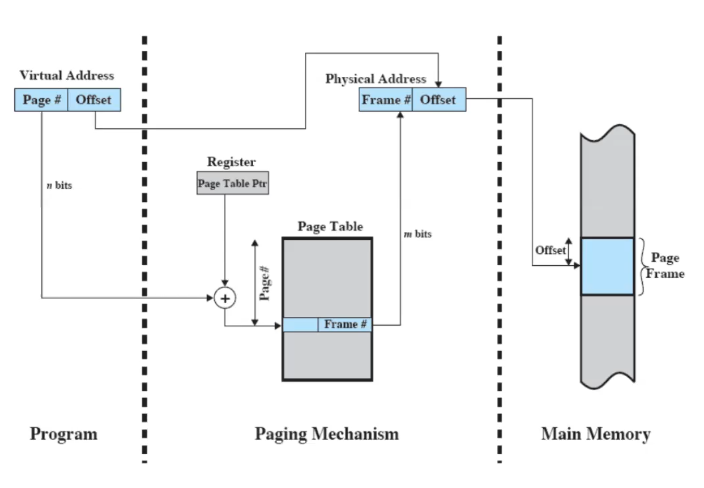
\includegraphics[width=0.65\textwidth]{immagini/HardwarePerPaginazione}
        \caption{Hardware Paginazione}
        \label{fig:hardwarepaginazione}
    \end{figure}
    Il sistema operativo deve :
    \begin{itemize}
        \item caricare a partire da un certo indirizzo / tabella delle pagine del processo
        \item caricare il valore di I in un opportuno registro dipendente dall'hardware
        \item questo va fatto per ogni process switch quindi fa sempre parte del passo 6
    \end{itemize}
    \subsubsection*{Tabelle delle pagine}
    Uno dei problemi é un overhead, perché le tabelle potrebbero contenere molti elmenti, quando un processo é in esecuzione
    , viene assicurato che almeno una parte della sua tabella sia in memoria principale. \\
    
    Esempio:
    \begin{itemize}
        \item Abbiamo 8GB di spazio virtuale, 1KB per pagina, \begin{math}2^23\end{math} entries per ogni tabella delle pagine, ovvero per ogni processo
        \item Con max 4GB di RAM, abbiamo 4 byte
        \item 4 byte per ogni entry 2^2^3=32MB per ogni processo
        \item quindi con 1 RAM di 1GB, bastano 20 processi per occupare piú della metá della memoria con sole strutture di
        overhead
    \end{itemize}
    \subsubsection*{Tabella delle pagine a 2 livelli}
    Per risolvere il problema dell'overhead, si puó usare una tabella delle pagine a 2 livelli, in cui la tabella delle
    pagine é divisa in due parti, la prima parte é una tabella di primo livello, che punta a delle tabelle di secondo livello
    \begin{Figure}
        \centering
        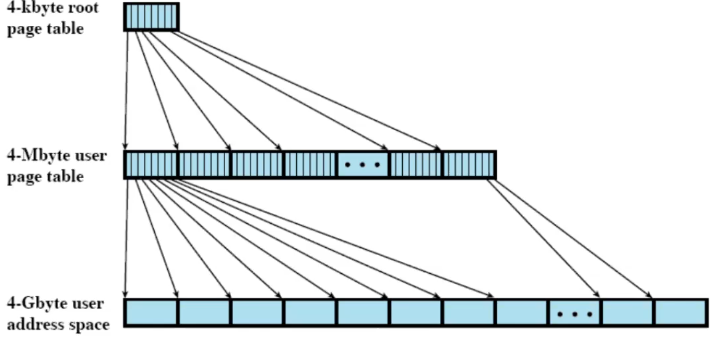
\includegraphics[width=0.65\textwidth]{immagini/TabellaA2Livelli}
        \caption{Tabella delle pagine a 2 livelli}
    \end{Figure}
    In questo caso l'indirizzo virtuale é diviso in 3 parti, la prima parte é usata per indicizzare la tabella di primo livello,
    la seconda parte é usata per indicizzare la tabella di secondo livello, e la terza parte é usata per indicizzare
    la pagina, in questo modo si riduce l'overhead.
    \begin{figure}
        \centering
        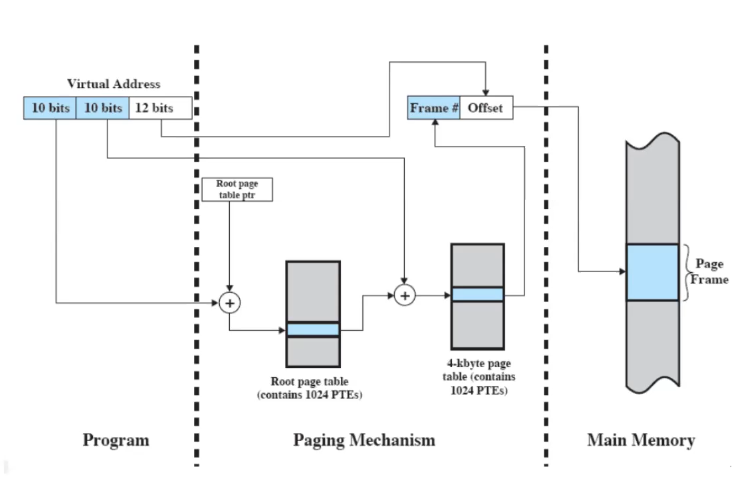
\includegraphics[width=0.65\textwidth]{immagini/HardwareTabella2Livelli}
        \caption{Hardware Tabella delle pagine a 2 livelli}
    \end{figure}
    \subsubsection{Translation Lookaside Buffer}
    IL TLB (memoria temporanea per la traduzione futura), ogni riferimento alla memoria virtuale puó generare
    due accessi alla memoria, si usa un cache veloce per gli elementi delle tabelle delle pagine.
    \subsubsection*{come funziona}
    Dato un indirizzo virtuale, il processore esamina il TLB, se l'indirizzo é presente, il TLB restituisce l'indirizzo
    altrimenti si prende la normale tabella delle pagine del processo,se la pagina risulta in memoria principale, si
    aggiorna il TLB, se la pagina non é in memoria principale, si genera un page fault e si carica in memoria ed infine
    viene aggiornato il TLB usando un algoritmo di sostituzione (LRU tipicamente).
    \begin{figure}[H]
        \centering
        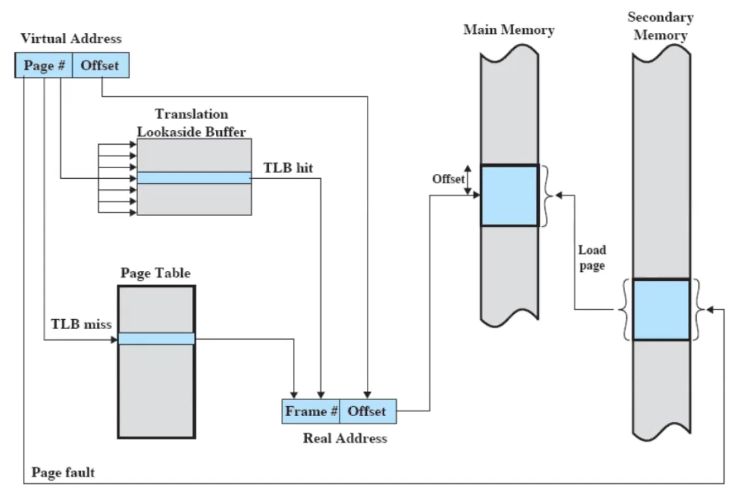
\includegraphics[width=0.65\textwidth]{immagini/HardwareTLB}
        \caption{TLB}
    \end{figure}
    \begin{figure}[H]
        \centering
        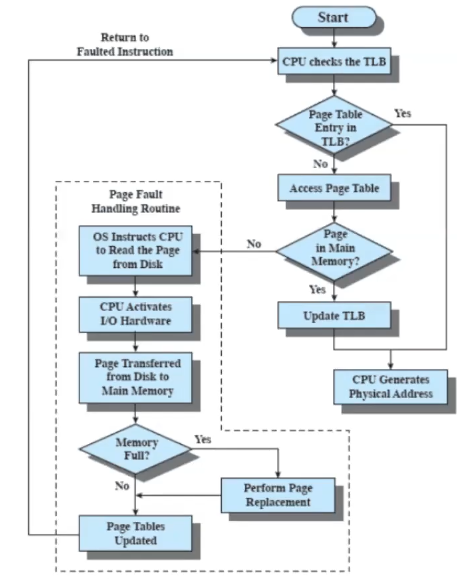
\includegraphics[width=0.65\textwidth]{immagini/FunzionamentoTLB}
        \caption{TLB}
    \end{figure}
    Il sistema operativo deve poter resettare il TLB, perché il TLB contiene informazioni di un processo, e se il processo
    cambia, il TLB deve essere resettato, alcuni processori permettono di avere il PID nel TLB, in modo da invalidare solo alcune
    parti del TLB, é comunque necessario anche senza TLB dire al processore dove é la nuova tabella delle pagine.
    \subsubsection*{Mapping Associativo}
    La tabella delle pagine ha tutte le entry, il TLB contiene solo alcune entry, quindi il numero della pagina non puó essere
    usato direttamente come indice per il TLB (possibile nella tabella delle pagine), Il SO inoltre puó interrogare piú
    elementi del TLB contemporaneamente per capire se c'é o no un hit \textbf{con il supporto hardware}, un altro
    problema é che bisogna fare in modo che il TLB contenga solo pagine in RAM, perché se ci fosse un page fault dopo
    un hit del TLB potremmo non accorgercene, quindi ogni volta che si swappa una pagina bisogna anche resettare o parzilemente il
    TLB.
    \begin{figure}[H]
        \centering
        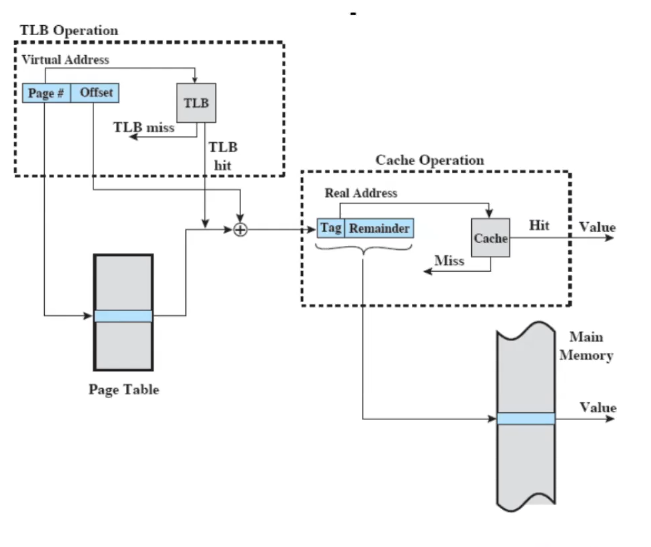
\includegraphics[width=0.65\textwidth]{immagini/TLBeCache}
        \caption{Mapping Associativo}
    \end{figure}
    \subsubsection{Dimensione delle pagine}
    Piú piccola é la pagina, minore é la frammentazione interna, ma maggiore é l'overhead, perché ci sono piú entry,
    la memoria secondaria é ottimizzata per trasferire grossi blocchi di dati, quindi avere le pagine ragionevolmente grandi
    non sarebbe male, quindi piú piccola é una pagina, maggiore il numero di pagine in RAM, E in tutte queste pagine, i riferimenti
    saranno vicini: in accordo con la localitá, i page fault saranno piú rari.
    \subsubsection*{Pagefault vs Dimensione delle pagine}
    \begin{figure}[H]
        \centering
        \includegraphics[width=0.65\textwidth]{immagini/Grafico1}
        \caption{Pagefault vs Dimensione delle pagine}
    \end{figure}
    Nelle moderne architetture HW possono supportare pagine anche fino ad 1GB, il sistema operativo
    ne sceglie 1 Es. Linux sugli x86 usa 4KB e le dimensioni piú grandi sono usati in sistemi operativi di grandi architetture
    clustes \ldotsecc ma anche per i sistemi operativi stessi(kernel Mode)















































\end{document}
